\documentclass[12pt,a4paper]{article}
\usepackage[margin=1in]{geometry}
\usepackage[utf8]{inputenc}
\usepackage{graphicx}
\usepackage{caption}
\usepackage[none]{hyphenat}
\usepackage{hyperref}
\usepackage[nameinlink]{cleveref}
\usepackage[table]{xcolor}
\usepackage[edges]{forest}

\definecolor{darkgreen}{RGB}{0, 150, 0}
\setlength{\fboxrule}{2pt}
\crefname{figure}{Figure}{Figures}

\begin{document}
	\begin{titlepage}
		
		\begin{center}
			
\includegraphics[width=0.5\textwidth]{QUT.jpg}\\
			[0.03\textheight]  
			\Large\textbf{Bachelor of IT (Computer Science)}\\
			\Large\textbf{Assignment 2 - Client-Side React Application}\\
			\large\textbf{CAB230 - Web Computing}\\
			[0.02\textheight]
			\large\textsl{Dane Madsen}\\
			\large\textsl{n10983864@qut.edu.au}
		\end{center}
		
	\end{titlepage}
	\tableofcontents
	\newpage
	
	\section{Introduction}
		\hyperref[subsec:appendixA]{\textbf{Appendix A}}
		\subsection{Purpose and Description}
			The purpose of this react application is to collate and display information regarding movies, 
			and cast members to the user in a responsive and accessible manner. The application should 
			allow the user to search for movies by year or title and display the results in a list (\cref{fig:figure1}).  
			When a movie is selected, the application should display all the details of the movie, 
			including the year the movie was made, the plot of the movie and all the cast members 
			involved with the movie (\cref{fig:figure2}). The application should also allow the user to visit individual 
			pages of cast members where the user can view that cast members details, including their 
			birth year, death year and all the movies they have been involved with.\\
			\\
			It achieve this goal and to provide the user with the best experience I can, i have used a 
			number of advanced react features, including the use of react router, IntesectionObserver and 
			react-responsive-carousel. The use of these features has allowed me to create a 
			professional looking application that is both easy to use and responsive for the user.\\
		
		\subsection{Completeness and Limitations}
			This implementation covers all the requirements of the assignment specification. 
			Navigation is handled using react router, controlled forms are used for all user input, and 
			every 10 minutes the refresh token is used to get a new access token. In addition to this, 
			the application uses ag-grid to display the search results in an infinitly scrolling grid 
			and react-responsive-carousel to display the highest scoring movies of all time on the 
			home (landing) page. On the person page the movies the person is involved in are displayed 
			in a grid with the IMDb Rating.\\

	\section{Use of End Points}
		\hyperref[subsec:appendixB]{\textbf{Appendix B}}\\
		\\
		The functionality for all the API endpoints is handled in API.js. This file contains all the 
		functions that are used to make requests to the API. By containing all the API functionality 
		in one file, it makes it easier to maintain and potentially update the application in the 
		future.\\

		\subsection{/movies/search}
			This endpoint is implemented as the getMovies function and is utilised by two 
			search forms at the top of the application. The first search form is for the user to search 
			for movies by title, and the second is for the user to search for movies by year. Both of 
			these forms are controlled forms and can be accessed from any page in the application. Doing 
			it this way removes an extra layer of complexity for the user and allows them to get into the 
			function of the application right from the start of	the application.\\
			(\cref{fig:figure3})

		\subsection{/movies/data/\{imdbID\}}
			This endpoint is implemented as the getMovie function and is utilised by the movie page to 
			get the details of the movie the user has selected. The movie page is accessed by clicking 
			on any of the movies in the search results. The movie page displays all the details of the 
			movie, including the title, year, box office earnings, runtime, genre, country of origin, 
			plot, cast and ratings. each cast member is a clickable link that will lead to that cast 
			members respective page.\\
			(\cref{fig:figure4})

		\subsection{/people/\{id\}}
			This endpoint is implemented as the getPerson function and is utilised by the person page 
			to get the details of the person the user has selected. The person page is accessed by 
			clicking on any of the cast members on the movie page. The person page displays all the 
			details of the person exposed by the API, including their name, birth year, death year, 
			all the movies they have been involved with. In a grid the name of each movie, the name 
			of the character the person played and the IMDb Rating is displayed for the users 
			convenience.\\
			(\cref{fig:figure5})

		\subsection{/user/register}
			This endpoint is implemented as the postRegister function and is utilised by the profile 
			page to register new users. The profile page is accessed by clicking on the profile button 
			in the navidation bar at the top of the page. When first launched, if the user isnt logged 
			in the profile page will be in the login state, if the user presses the register button the 
			profile page will be transitioned into the register state. The register state contains 
			fields for the user to enter their email, password and confirm password. If the user 
			presses the register button the /user/register endpoint will be utilised to register the 
			user and the tokens will be stored in local storage. If the user presses back to login the 
			page will be transitioned back into the login state.\\
			(\cref{fig:figure6})

		\subsection{/user/login}
			This endpoint is implemented as the postLogin function and is utilised by the profile page 
			to login existing users. If the user accesses the the profile page while logged out they 
			will be gretted with a login prompt with an email and password field, button to login and 
			a button to register. If the user presses the register button the page will be transitioned 
			into the register state. If the user presses the login button the /user/login endpoint will 
			be utilised to login the user and the tokens will be stored in local storage.\\
			(\cref{fig:figure7})

		\subsection{/user/refresh}
			This endpoint is implemented as the postRefresh function and is utilised in the back end 
			in App.js to refresh the tokens when the app first starts and every 10 minutes after. 
			This is done to ensure the user does not have to login every 10 minutes.
		
		\subsection{/user/logout}
			This endpoint is implemented as the postLogout function and is utilised by the profile 
			page to logout the user. If the user accesses the the profile page while logged in they 
			will be greeted with a message telling them they are logged in accompanied with a button 
			to logout, if the user presses the logout button the /user/logout endpoint will be utilised 
			to logout the user and the tokens will be deleted.\\
			(\cref{fig:figure8})

	\section{Modules Used}
		\subsection{react-router-dom}
			This module was used to handle navigation within the application. It was used to create 
			the navigation bar at the top of the page and to create the routes for the different 
			pages in the application.\\

			\href{https://www.npmjs.com/package/react-router-dom}{https://www.npmjs.com/package/react-router-dom}
		
		\subsection{react-responsive-carousel}
			This module was used to create a carousel on the home page to display the movies with the 
			highest IMDb Rating.\\

			\href{https://www.npmjs.com/package/react-responsive-carousel}{https://www.npmjs.com/package/react-responsive-carousel}
		
		\subsection{ag-grid-react}
			This module was used in MoviesPage to create a grid to display the search results in an infinitely 
			scrolling grid, and in PersonPage it is used to display the movies the person stars in.\\

			\href{https://www.npmjs.com/package/ag-grid-react}{https://www.npmjs.com/package/ag-grid-react}
		
		\subsection{ag-grid-community}
			This module was used in both MoviesPage and PersonPage to utilise the CSS for the respective grids.\\

			\href{https://www.npmjs.com/package/ag-grid-community}{https://www.npmjs.com/package/ag-grid-community}
	
	\newpage

	\section{Application Design}
		\hyperref[subsec:appendixC]{\textbf{Appendix C}}
		\subsection{Navigation and Layout}
			The application has been designed to be as simple to use as possible. The ultimate goal of the 
			design was to develop a user experience that the user can understand and use without having to 
			think about it.\\
			\\
			A few design choices were made to achive this goal. The first major choice i made was to move the 
			search bars to the navigation bar at the top of the page. This was done to make the search 
			functionality more accessible to the user by allowing them to search from any page in the 
			application. Moving the search bars to the navigation also freed up space on the MoviesPage 
			allowing me to display more search results at once.\\

			During development i also investigated the possibility of having the poster image for each movie 
			displayed in the search results (\cref{fig:figure10}, \cref{fig:figure11}). I decided against this 
			as it excessively queries the API and often resulted in a rate limit. It also increased the complexity 
			of being able to sort the search results which was something I wanted to implement.\\

		\subsection{Usability and Quality of Design}
			As the application was designed with simplicity in mind, the usability of the application is 
			very high. The application is very easy to use and the user can navigate the application with 
			ease. The application is layed out in a way that is very clean, the only page that can at all be 
			considered cluttered is the LandingPage because of the carousel but even then the carousel is 
			very clean, easy to use and it doesnt seems to distract the user from the rest of the page.\\
			\\
			The navigation of the app is very simple and easy for the user to understand. As previously mentioned, 
			by having the search bars within  the navigation bar at the top of the page the user can search from 
			anywhere in the application. The only part of the navigation that may confuse the user is the home button 
			using the logo of the application. It may not be clear to the user that this is a button that leads them 
			home. But, this is quite a common design choice in web design and there isnt much use for the user to return 
			to the home page as the user can search from any page in the application.\\
			\\
			The design of the application is consistent throughout. The navigation bar is the same on every page, 
			very little colours are used throughout the application and the colours that are used are consistent.
			Only the standard font is used throughout the application except in the ag-grids where a seperate style 
			is used.\\
		
		\subsection{Accessibility}
			The application has attempted to be as accessible as possible. The application achieve most of the 
			checkpoints of the W3C Web Content Accessibility Guidelines 2.0. The application has achived the 
			following checkpoints:
			\begin{itemize}
				\item 1.1.1 All non-text content such as images have alternative text.
				\item 1.2.1 Information conveyed in colour can also be conveyed in black and white. 
				\item 1.6.1 Page can be read without CSS.
				\item 1.6.2 Text equivalents update when content changes.
				\item 1.7.1 The screen doesnt flicker.
				\item 1.14.1 The application uses the clearest language appropriate.
			\end{itemize}
		
	\section{Technical Description}
		\subsection{Architecture}
			\begin{itemize}
				\item \textbf{Components:}\\
					This folder contains the components and the API handler for the application.
				\item \textbf{Pages:}\\
					This folder contains all the pages for the application.
				\item \textbf{Styles:}\\
					This folder contains all the CSS files for the application.
		  	\end{itemize}
			The diagram on the next page show the file structure of the application. As you can see, the 
			application is structured in a very simple way. As previously mentioned, all the code for 
			handling API requests is contained within the API.js file. This has made it easier to write 
			the code for the application as it is all in one place and can be reused easily.\\
			
			The only component of the application that has been seperated out into its own file is the 
			search inputs. The only reason this was done was because I couldnt get it working within 
			App.js.\\

			Each page of the application has its own JS and CSS file. This was done to make the code 
			easier to read and understand, and to cut down on the amount of code in each file.\\	
		
			\begin{minipage}[b]{0.5\textwidth}
				\begin{forest}
					for tree={
					  folder,
					  grow'=0,
					  fit=band,
					}
					[Project Root
						[Docs]
						[Public]
						[SRC]
						[.gitignore]
						[package-lock.json]
						[package.json]
						[README.md]
					]
				\end{forest}
			\end{minipage}
			\hfill
			\begin{minipage}[c]{0.5\textwidth} 
				\begin{forest}
				for tree={
				  folder,
				  grow'=0,
				  fit=band,
				}
				[SRC
				  [Components
					[SearchInputs.js]
					[API.js]
				  ]
				  [Pages
					[LandingPage.js]
					[MoviePage.js]
					[MoviesPage.js]
					[PersonPage.js]
					[ProfilePage.js]
				  ]
				  [Styles
					[App.css]
					[LandingPage.css]
					[MoviePage.css]
					[MoviesPage.css]
					[PersonPage.css]
					[ProfilePage.css]
					[SearchInputs.css]
				  ]
				  [App.js]
				  [Logo.svg]
				]
			  \end{forest}
			\end{minipage}
			\newpage
		\subsection{Test Plan}
			\hyperref[subsec:appendixD]{\textbf{Appendix D}}\\
			\\
			\begin{tabular}{|p{0.3\textwidth}|p{0.4\textwidth}|p{0.08\textwidth}|p{0.22\textwidth}|}
				\hline
				\rowcolor{gray!30}
				\textbf{Task} & 
				\textbf{Expected Outcome} & 
				\textbf{Result} & 
				\textbf{Screenshot} \\
				\hline
				Search by title. & 
				List of movies returned & 
				\textcolor{darkgreen}{PASS} & 
				\cref{fig:figure13} \\
				\hline
				Search by year. & 
				List of movies returned & 
				\textcolor{darkgreen}{PASS} & 
				\cref{fig:figure14} \\
				\hline
				Search by title and year. &
				Movie, or List of movies returned & 
				\textcolor{darkgreen}{PASS} &
				\cref{fig:figure15} \\
				\hline
				Click on a movie. &
				Respective movie page is displayed. &
				\textcolor{darkgreen}{PASS} &
				\cref{fig:figure16} \\
				\hline
				Click on a cast member.
				(Logged Out) &
				User is prompted to Login &
				\textcolor{darkgreen}{PASS} &
				\cref{fig:figure17} \\
				\hline
				Click on a cast member.
				(Logged In) &
				Respective person page is displayed. &
				\textcolor{darkgreen}{PASS} &
				\cref{fig:figure18} \\
				\hline
				Register a new user. &
				User is registered and logged in. &
				\textcolor{darkgreen}{PASS} &
				\cref{fig:figure19} 
				\cref{fig:figure20} \\
				\hline
				Login as a user. &
				User is logged in. &
				\textcolor{darkgreen}{PASS} &
				\cref{fig:figure21}
				\cref{fig:figure22} \\
				\hline
				Log out as a user. &
				User is logged out. &
				\textcolor{darkgreen}{PASS} &
				\cref{fig:figure23} 
				\cref{fig:figure24} \\
				\hline
			\end{tabular}
	
		\subsection{Difficulties, Exclusions or Unresolved and Persistent Errors}
			The only notable issues that persist in the final version of the app is the lack of 
			an ability to sort the movies by title, year or rating, and an error that occurs when the 
			application has been offline for more than a day. The first issue is due to the fact that 
			the API doesnt support sorting and the second issue is due to the fact that the refresh 
			token expires after 24 hours. In summation, both of these issues are server side so theres 
			not alot that can be done.\\
	
	\section{User Guide}

	\newpage

	\section{Appendix}
		\subsection{Appendix A - Introduction}
		\label{subsec:appendixA}
			\begin{center}
			  	\fbox{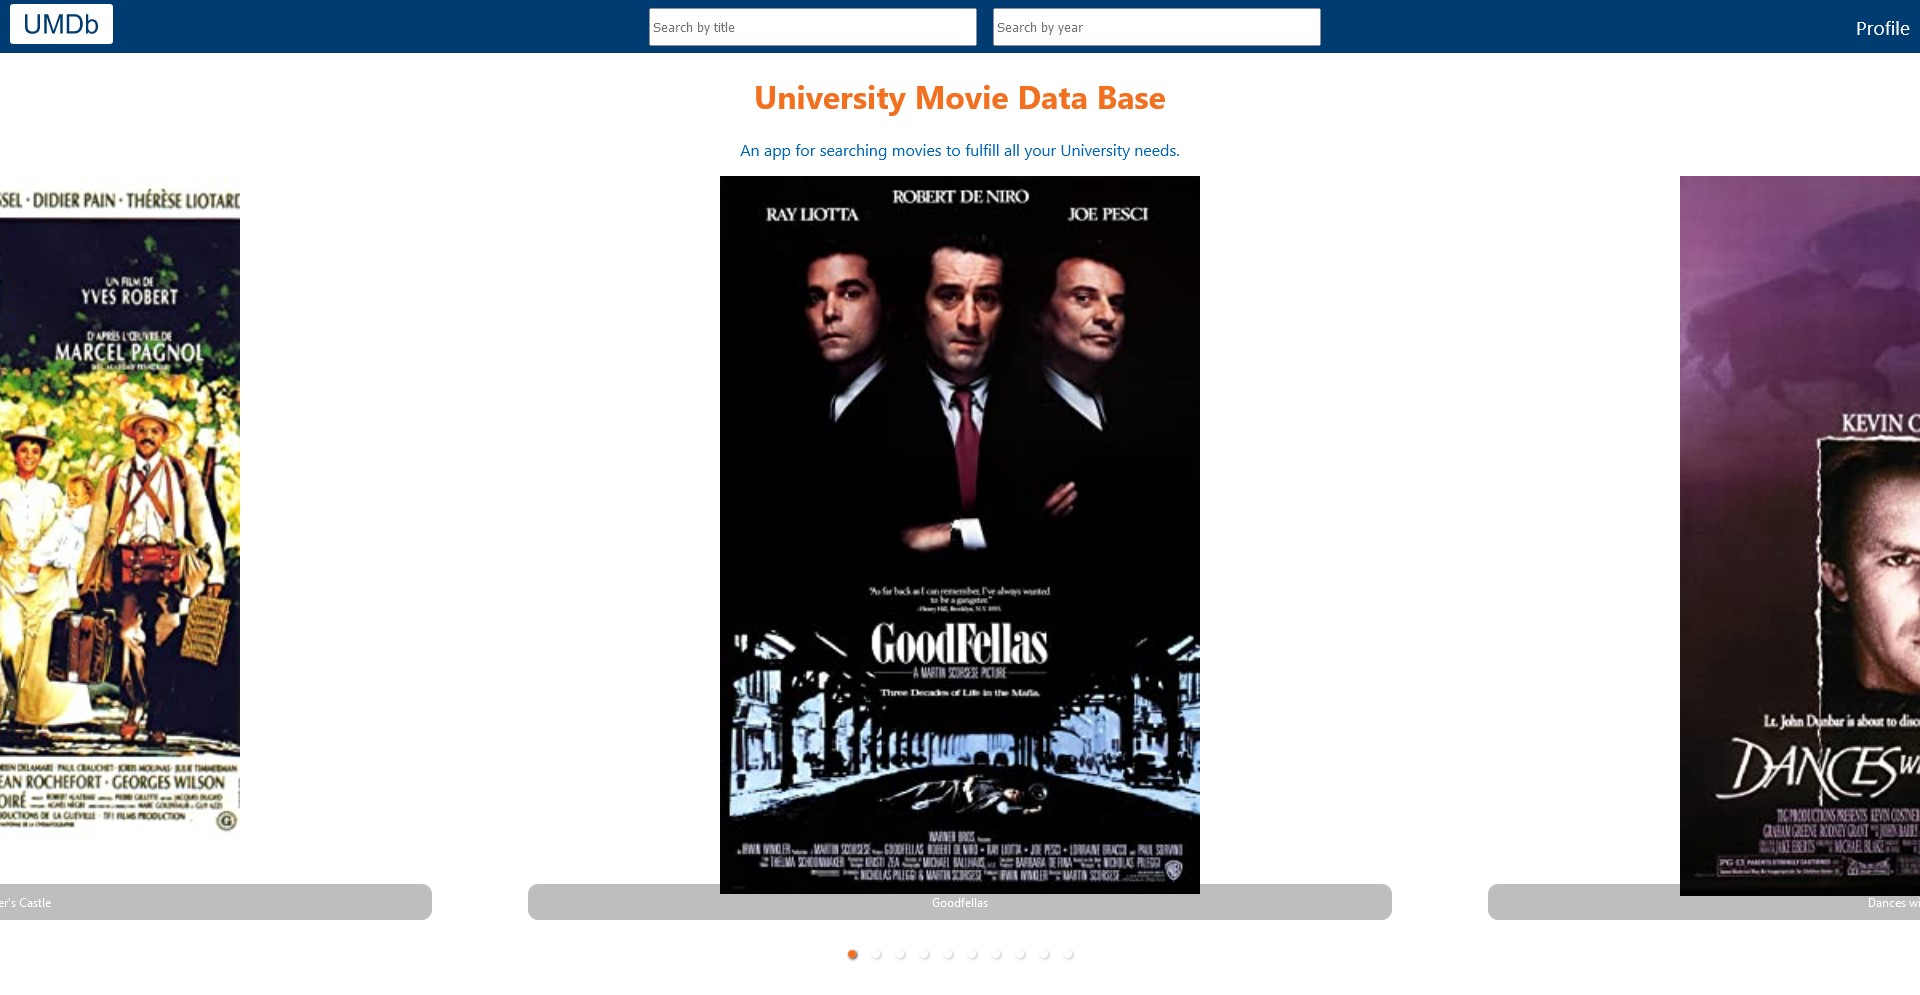
\includegraphics[width=\textwidth]{./figures/Figure1.jpg}}
			  	\captionof{figure}{Landing Page of the Application}
			  	\label{fig:figure1}
			  	\vspace{10pt}
			  	\fbox{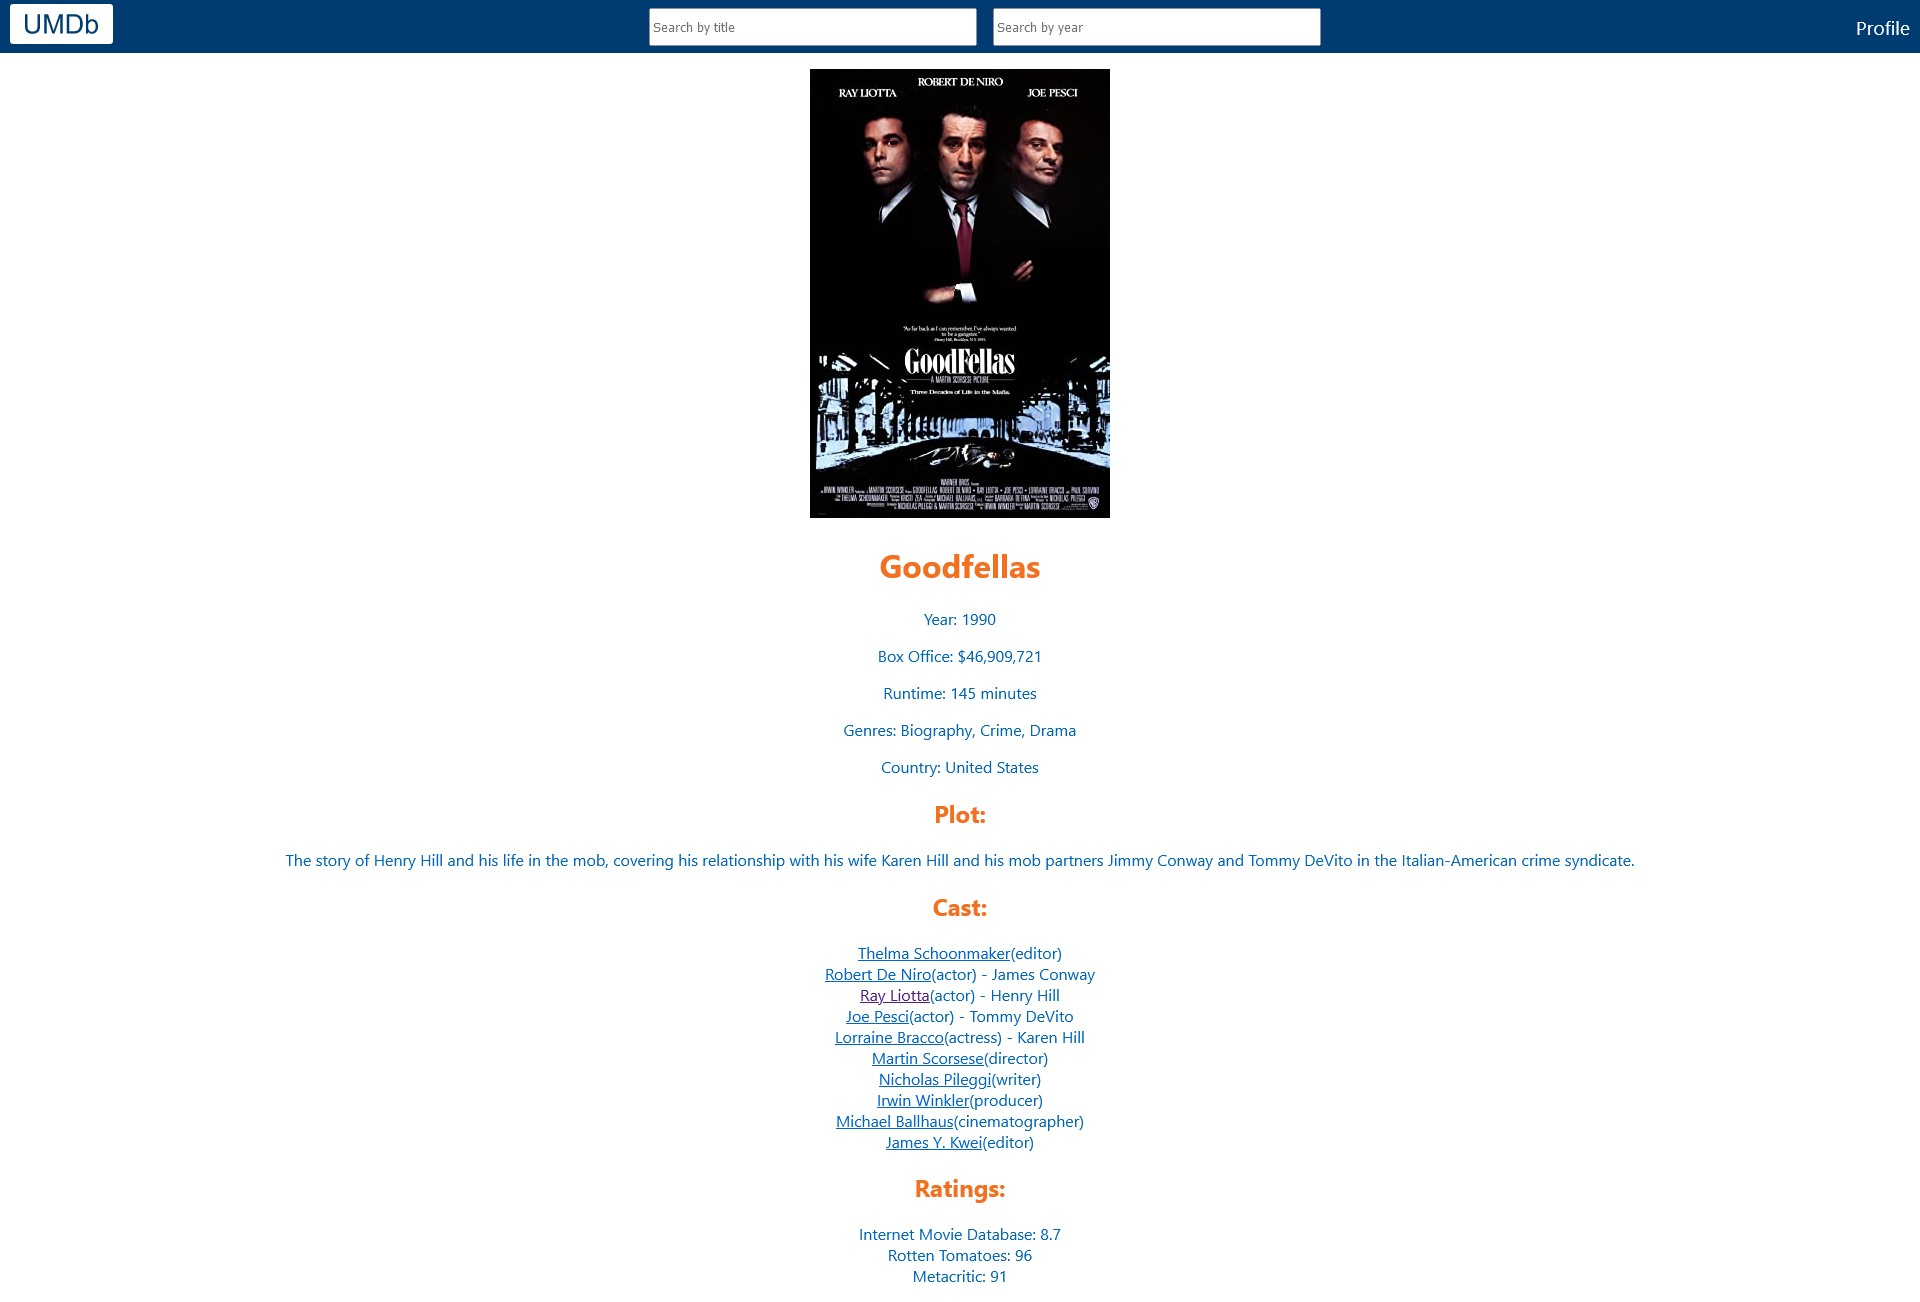
\includegraphics[width=\textwidth]{./figures/Figure2.jpg}}
			  	\captionof{figure}{Movie Page of the Movie "Goodfellas"}
			  	\label{fig:figure2}
				\vspace{10pt}
			  	\fbox{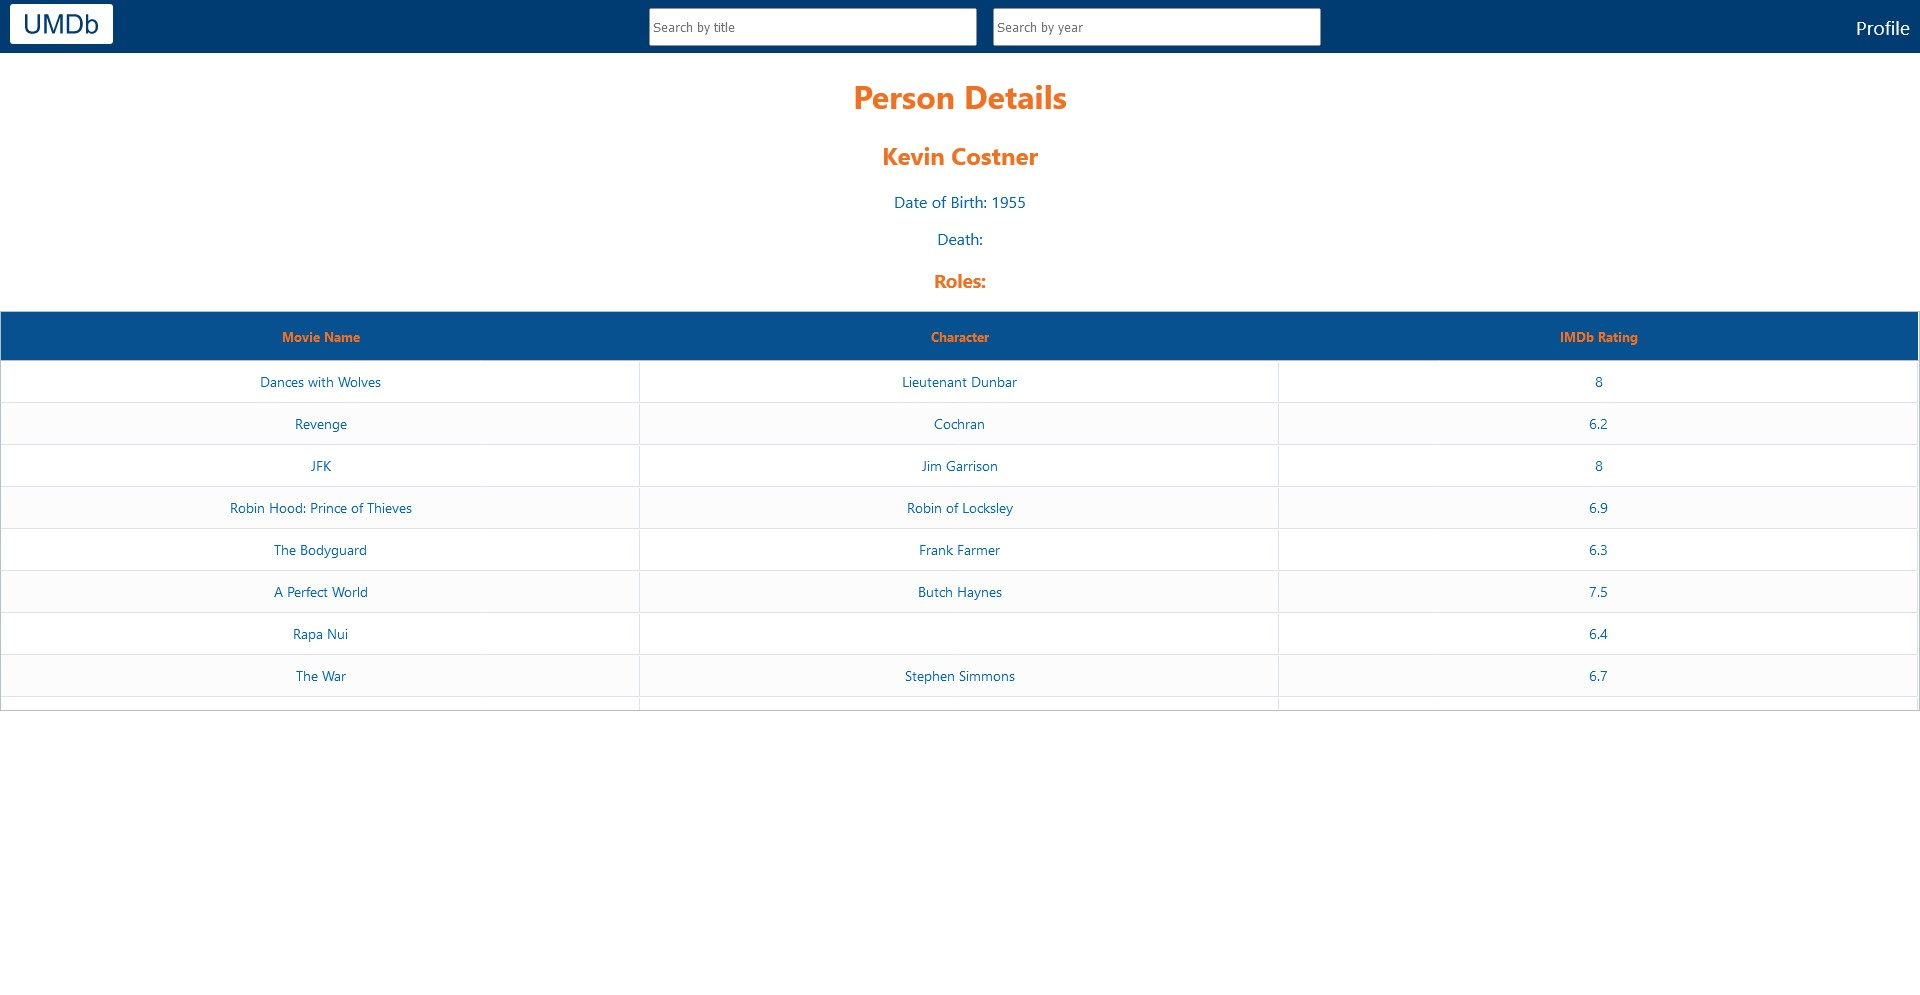
\includegraphics[width=\textwidth]{./figures/Figure3.jpg}}
			  	\captionof{figure}{Person Page of the Actor "Kevin Costner"}
			  	\label{fig:figure3}
			\end{center}
		\subsection{Appendix B - Use of End Points}
		\label{subsec:appendixB}
			\begin{center}
			  	\fbox{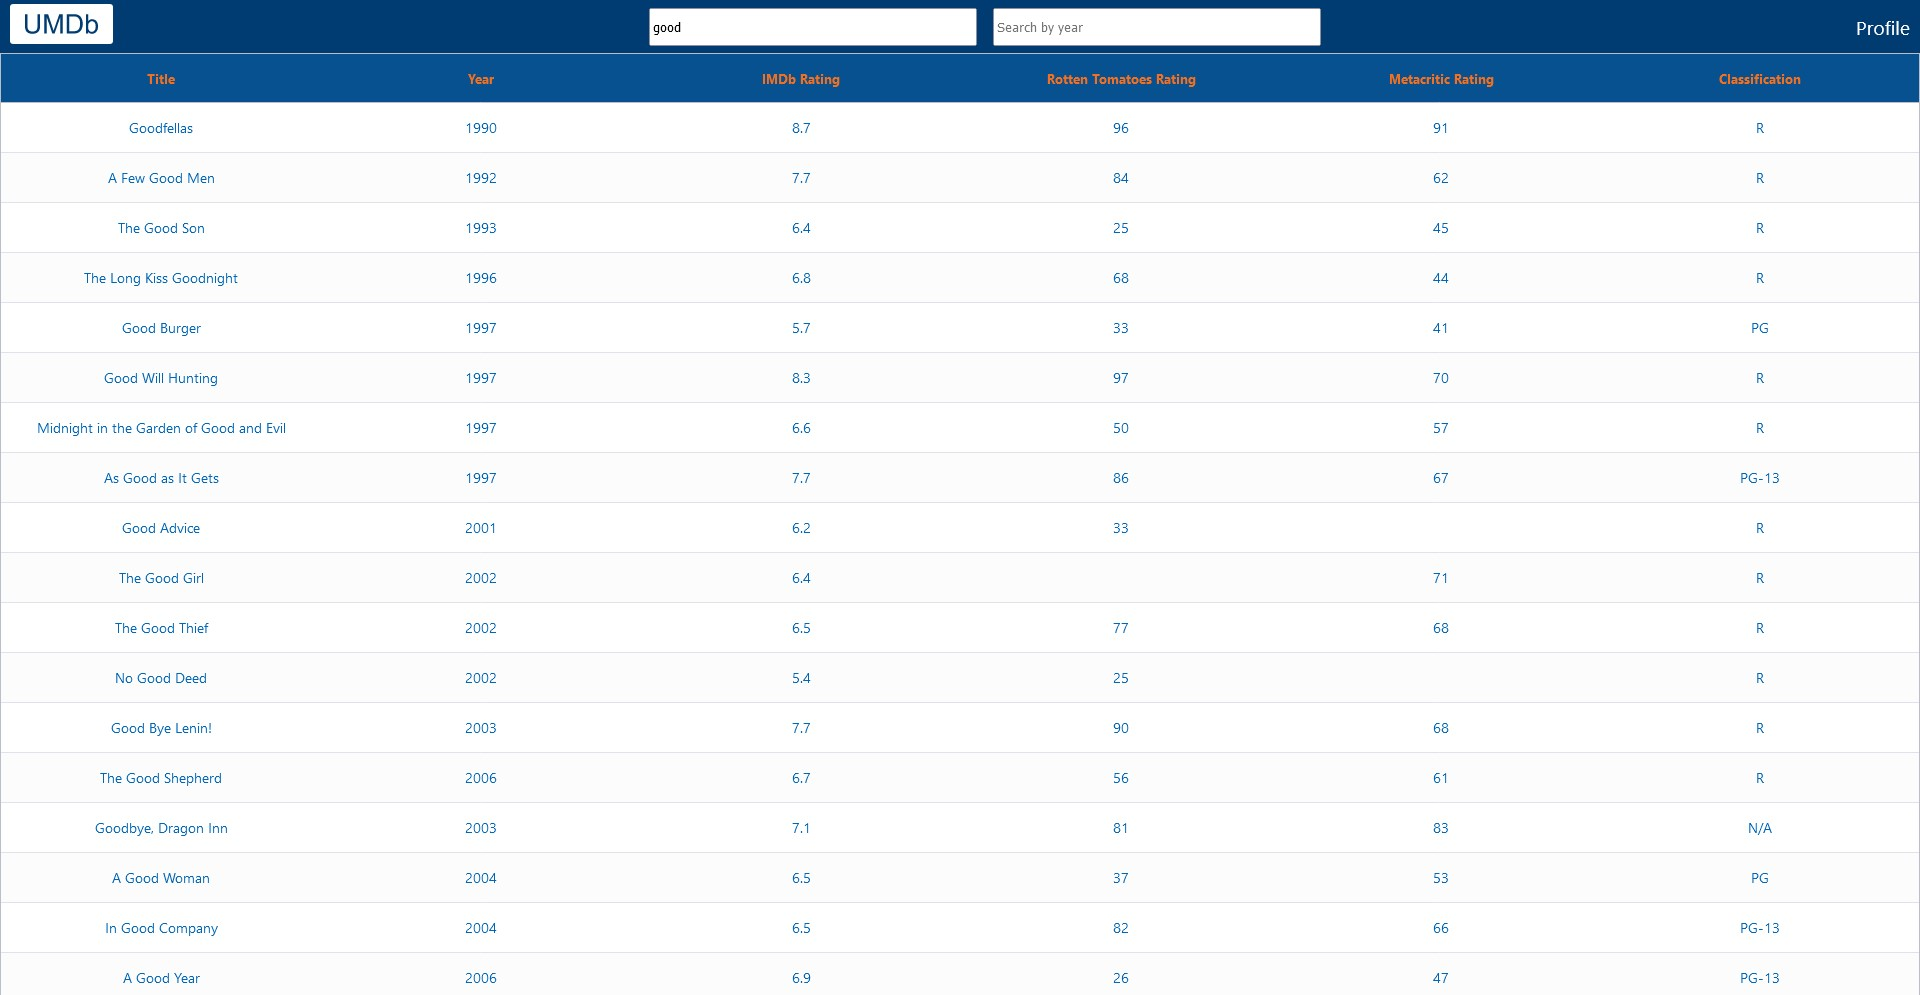
\includegraphics[width=\textwidth]{./figures/Figure4.jpg}}
			  	\captionof{figure}{Movies Page of the Application}
			  	\label{fig:figure4}
			  	\vspace{10pt}
			  	\fbox{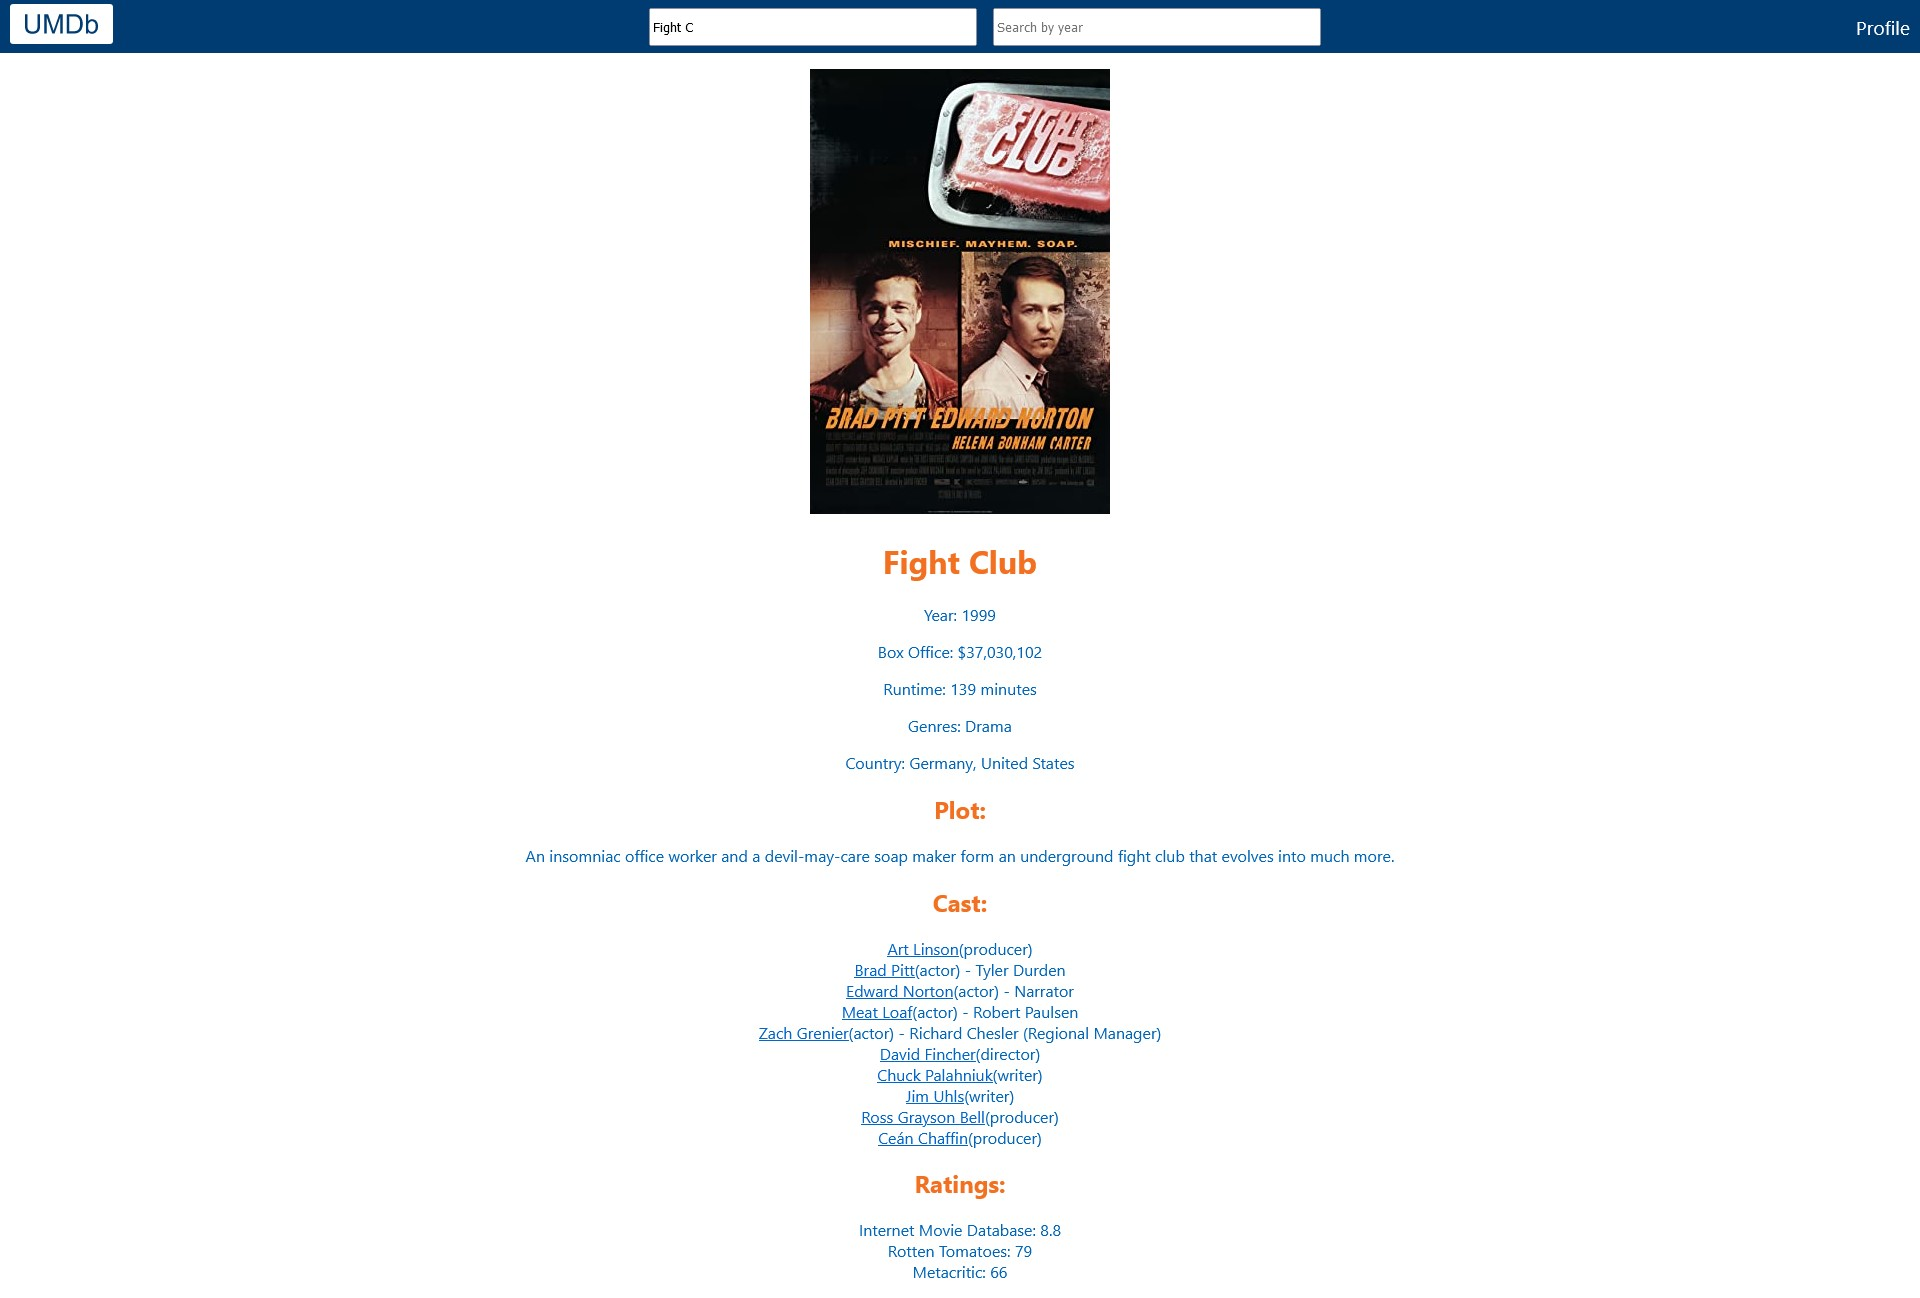
\includegraphics[width=\textwidth]{./figures/Figure5.jpg}}
			  	\captionof{figure}{Movie Page of the Movie "Fight Club"}
			  	\label{fig:figure5}
			  	\vspace{10pt}
			  	\fbox{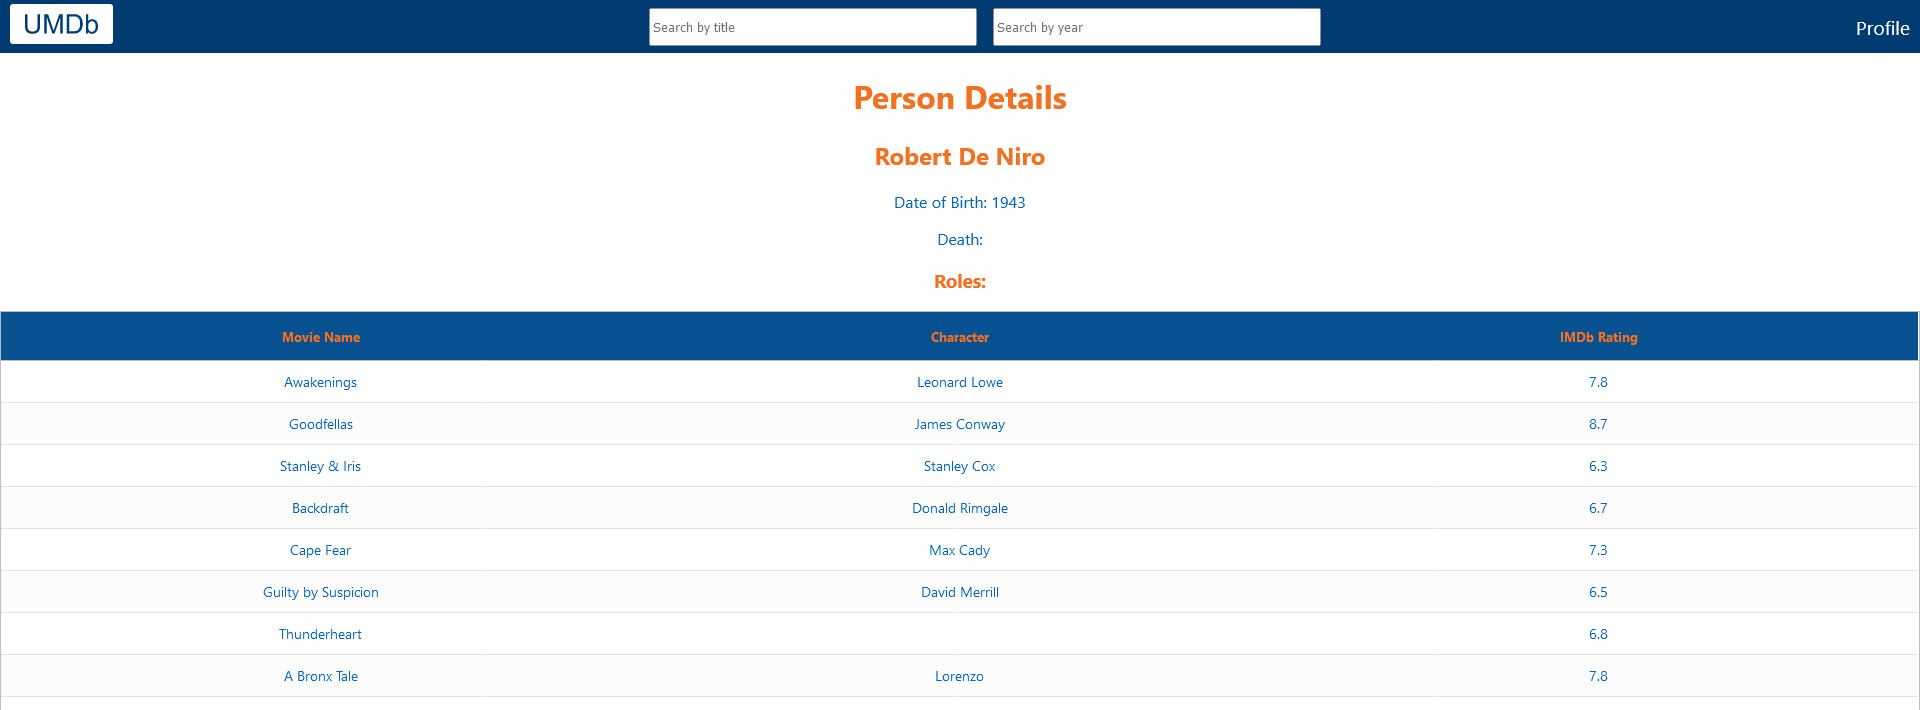
\includegraphics[width=\textwidth]{./figures/Figure6.jpg}}
			  	\captionof{figure}{Person Page of the Actor "Robert De Niro"}
			  	\label{fig:figure6}
				\vspace{10pt}
				\fbox{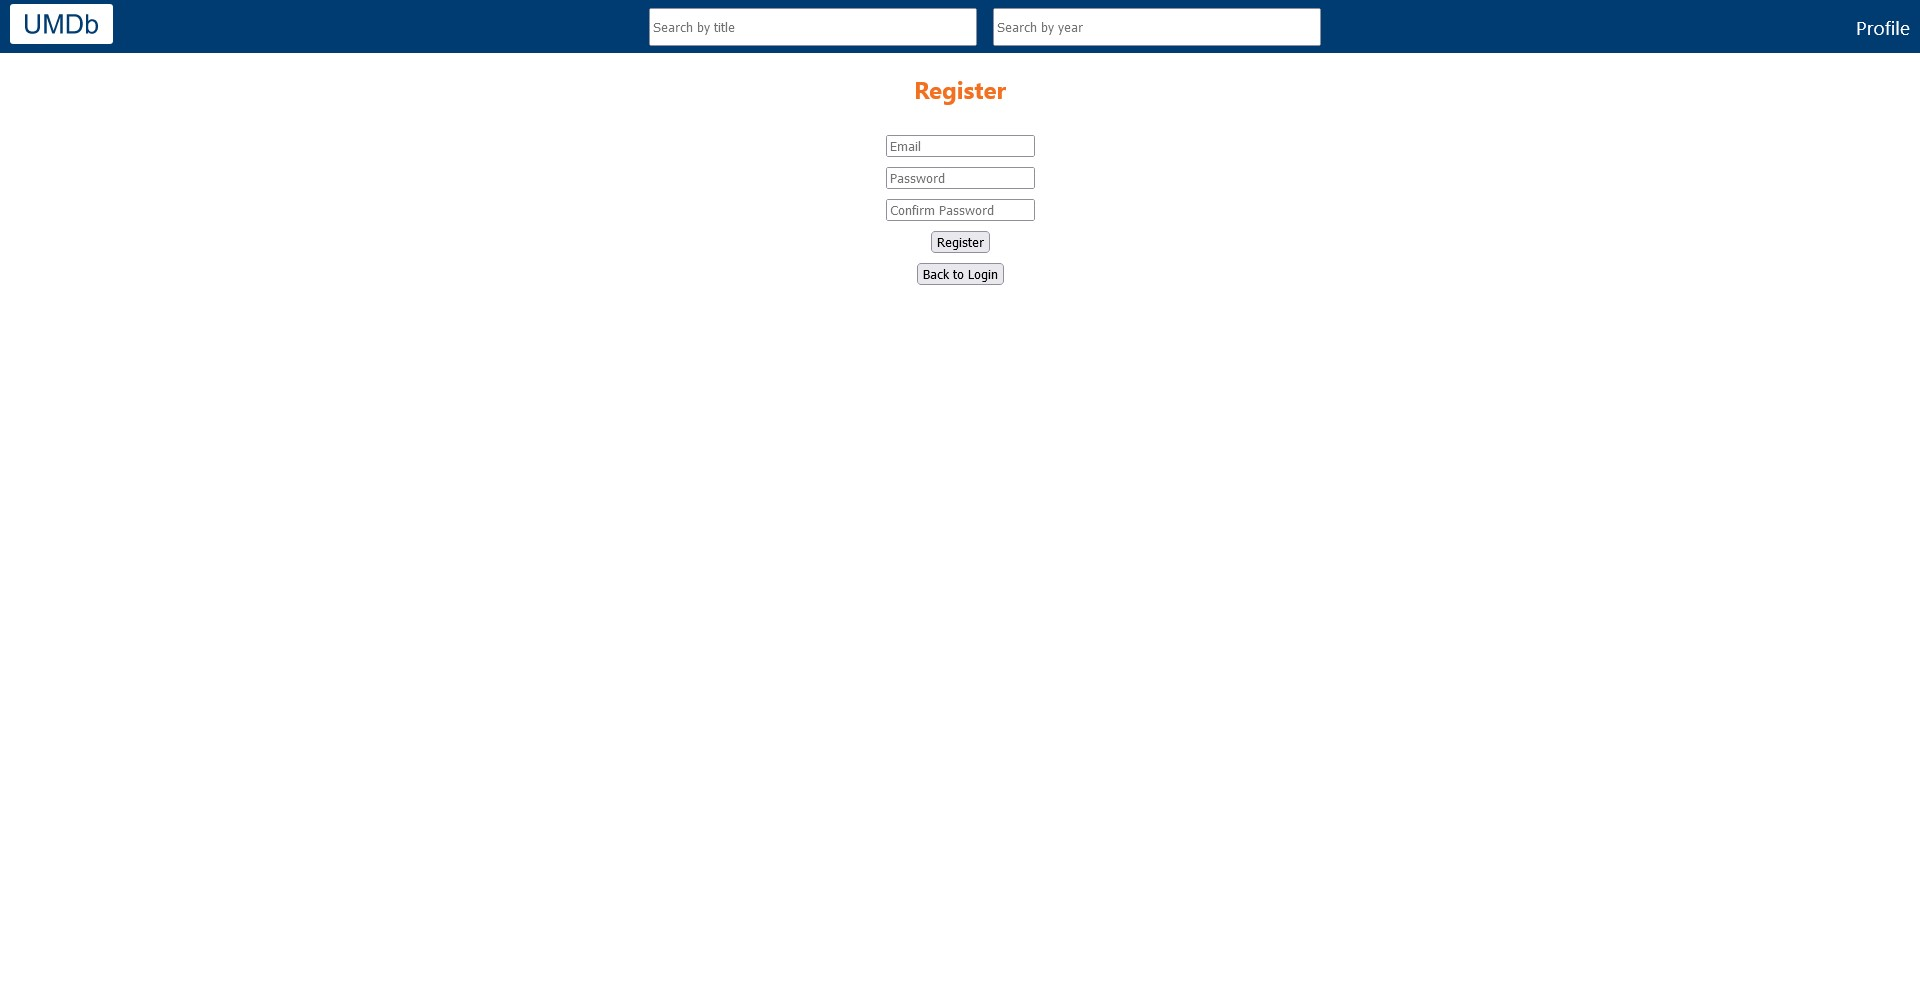
\includegraphics[width=\textwidth]{./figures/Figure7.jpg}}
			  	\captionof{figure}{Profile Page in the Register State}
			  	\label{fig:figure7}
				\vspace{10pt}
				\fbox{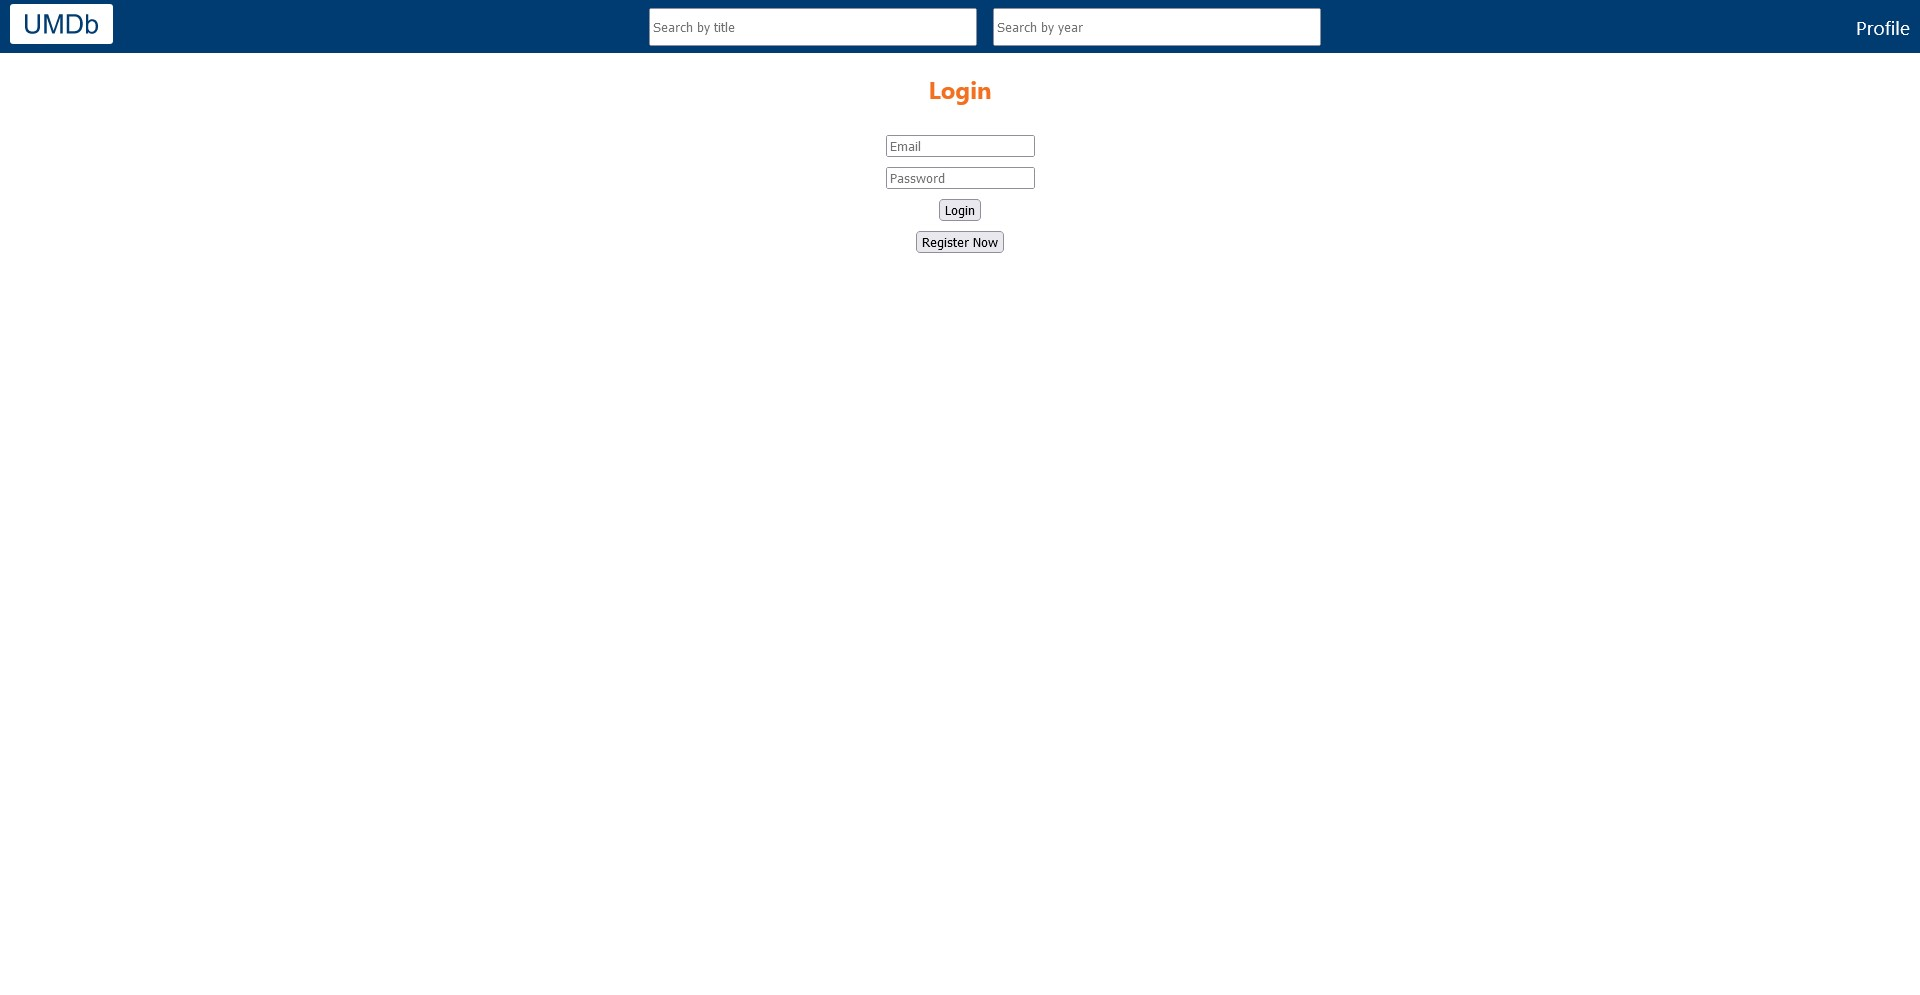
\includegraphics[width=\textwidth]{./figures/Figure8.jpg}}
			  	\captionof{figure}{Profile Page in the Login State}
			  	\label{fig:figure8}
				\vspace{10pt}
				\fbox{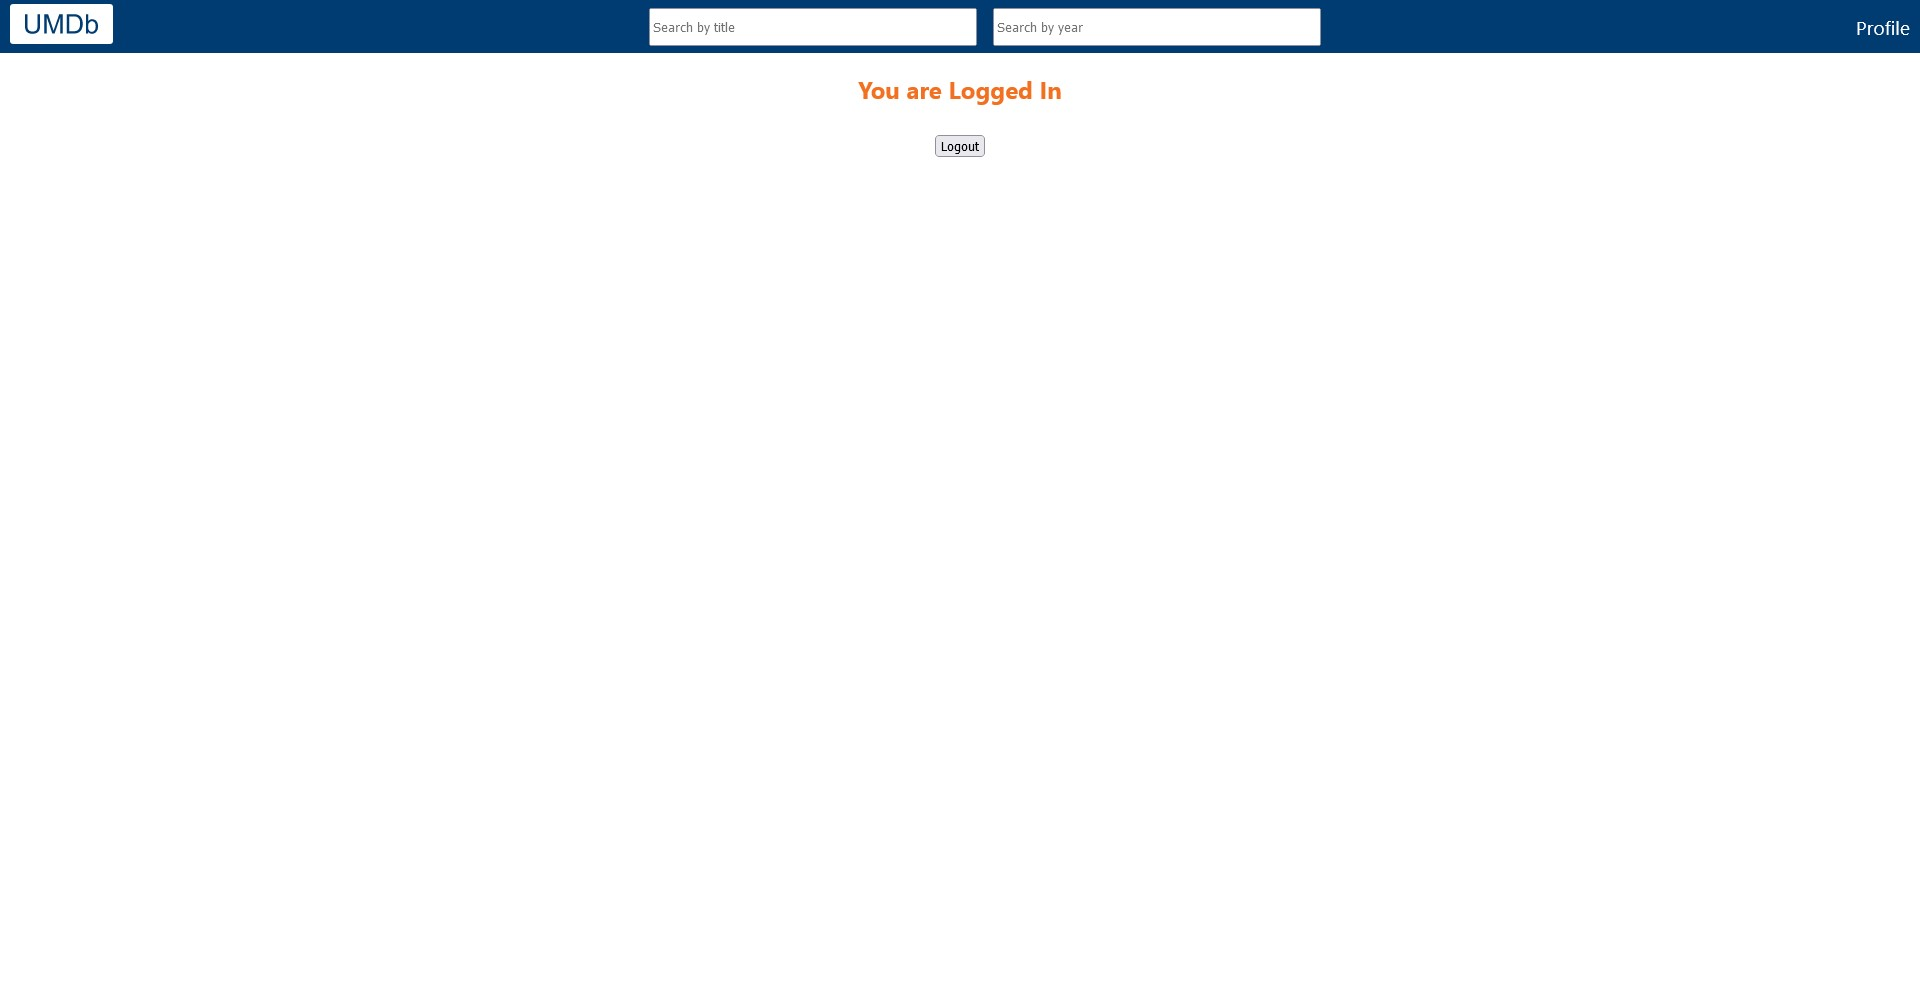
\includegraphics[width=\textwidth]{./figures/Figure9.jpg}}
			  	\captionof{figure}{Profile Page Ready for the User to Logout}
			  	\label{fig:figure9}	
			\end{center}
		\subsection{Appendix C - Application Design}
		\label{subsec:appendixC}
			\begin{center}
			  	\fbox{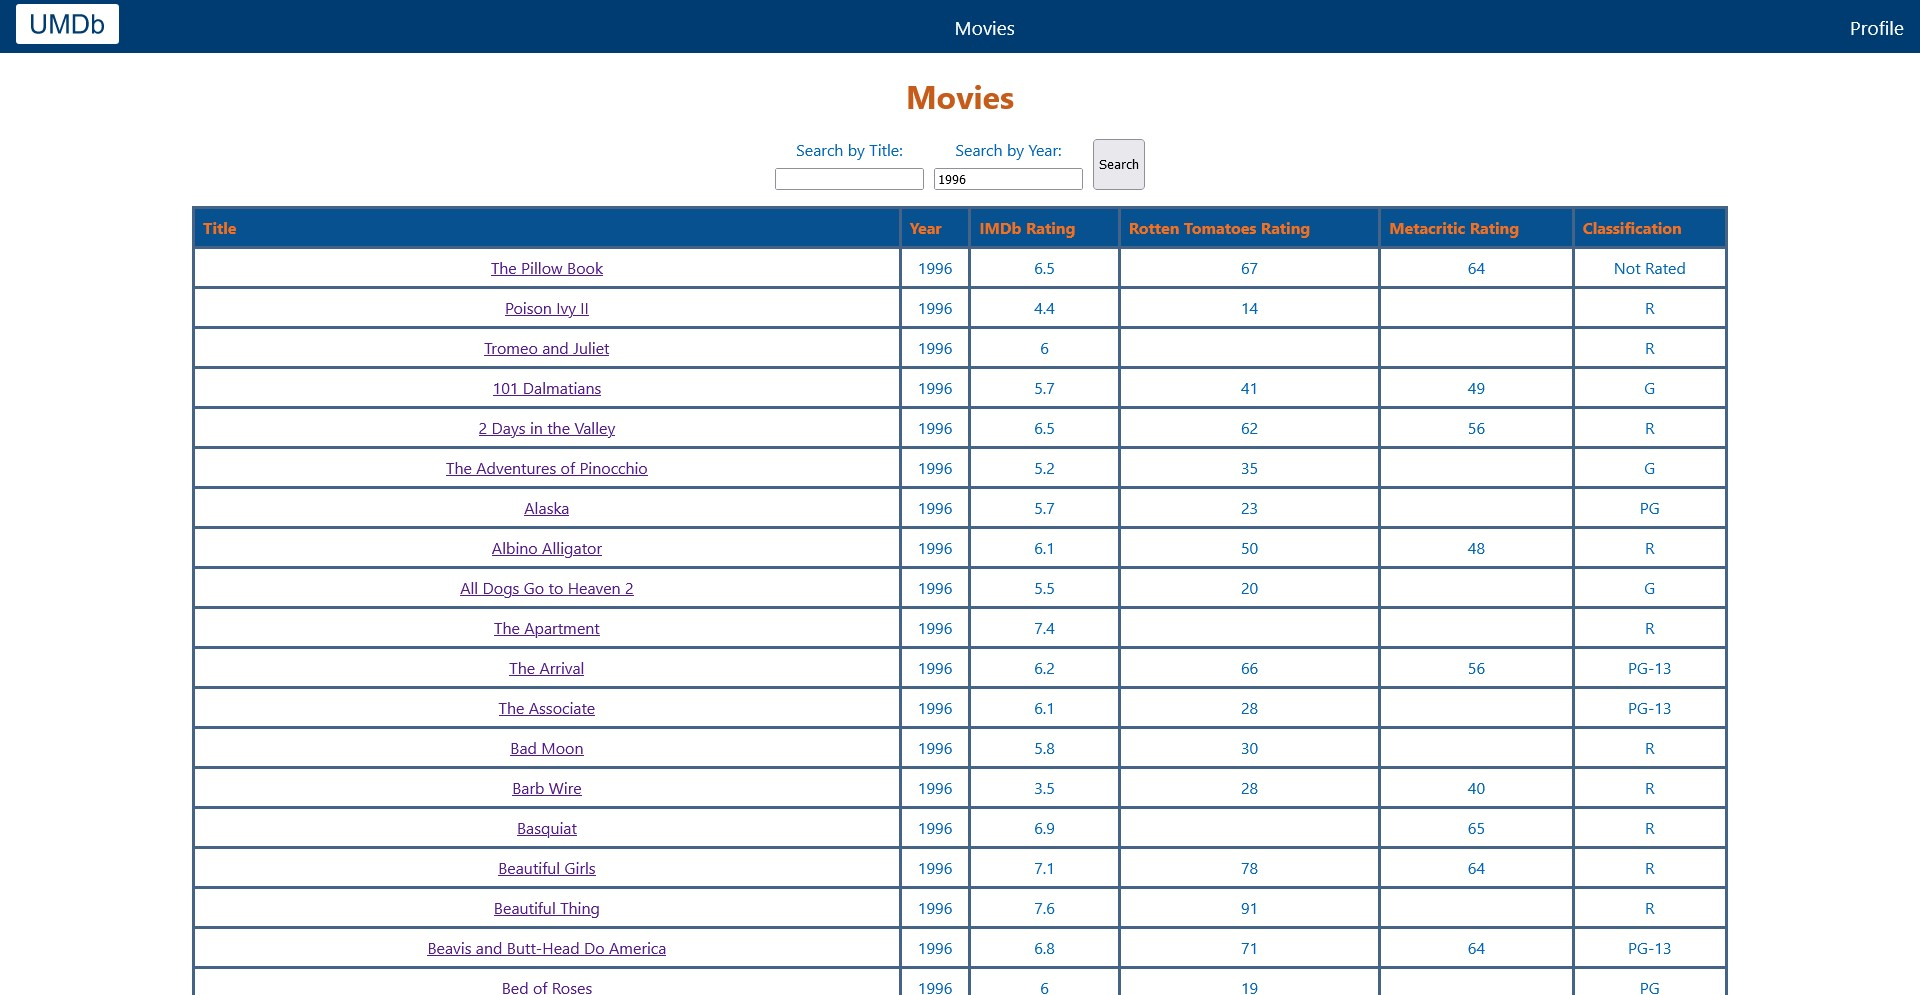
\includegraphics[width=\textwidth]{./figures/Figure10.jpg}}
			  	\captionof{figure}{An earlier version of the MoviePage}
			  	\label{fig:figure10}
			  	\vspace{10pt}
			  	\fbox{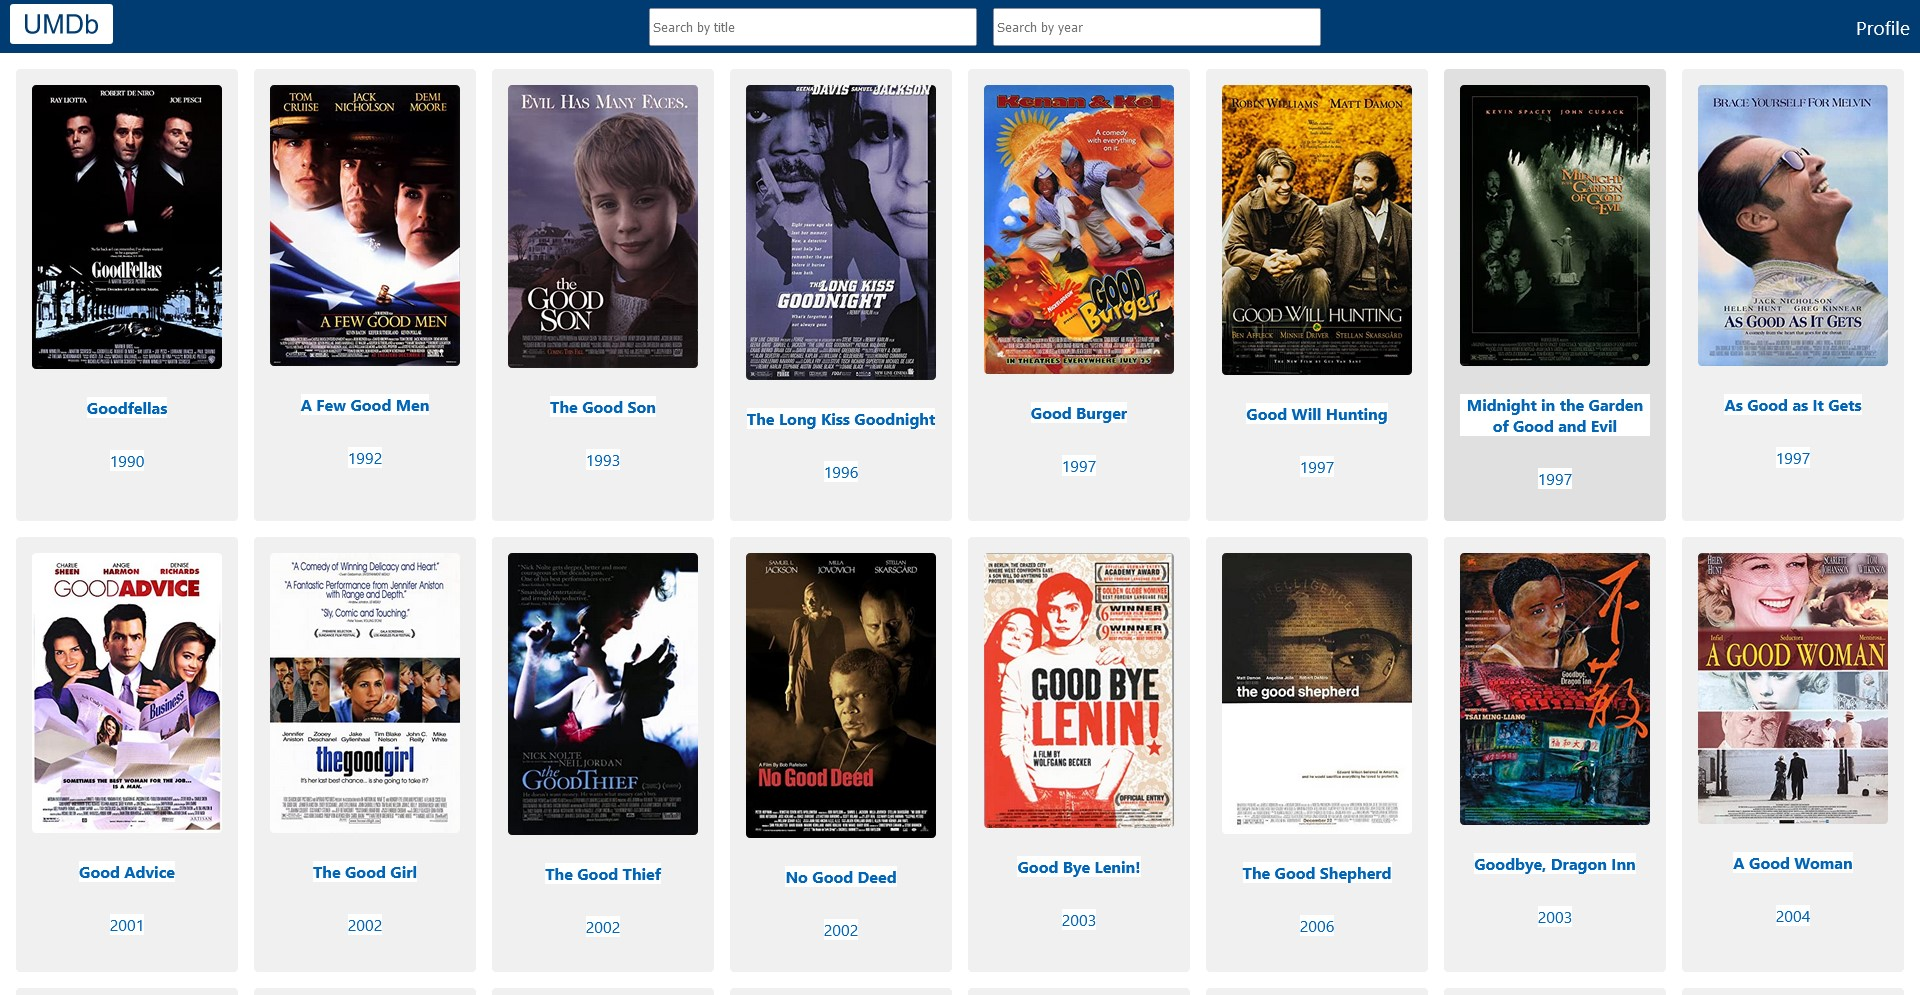
\includegraphics[width=\textwidth]{./figures/Figure11.jpg}}
			  	\captionof{figure}{An experimental version of the MoviesPage}
			  	\label{fig:figure11}
			  	\vspace{10pt}
			  	\fbox{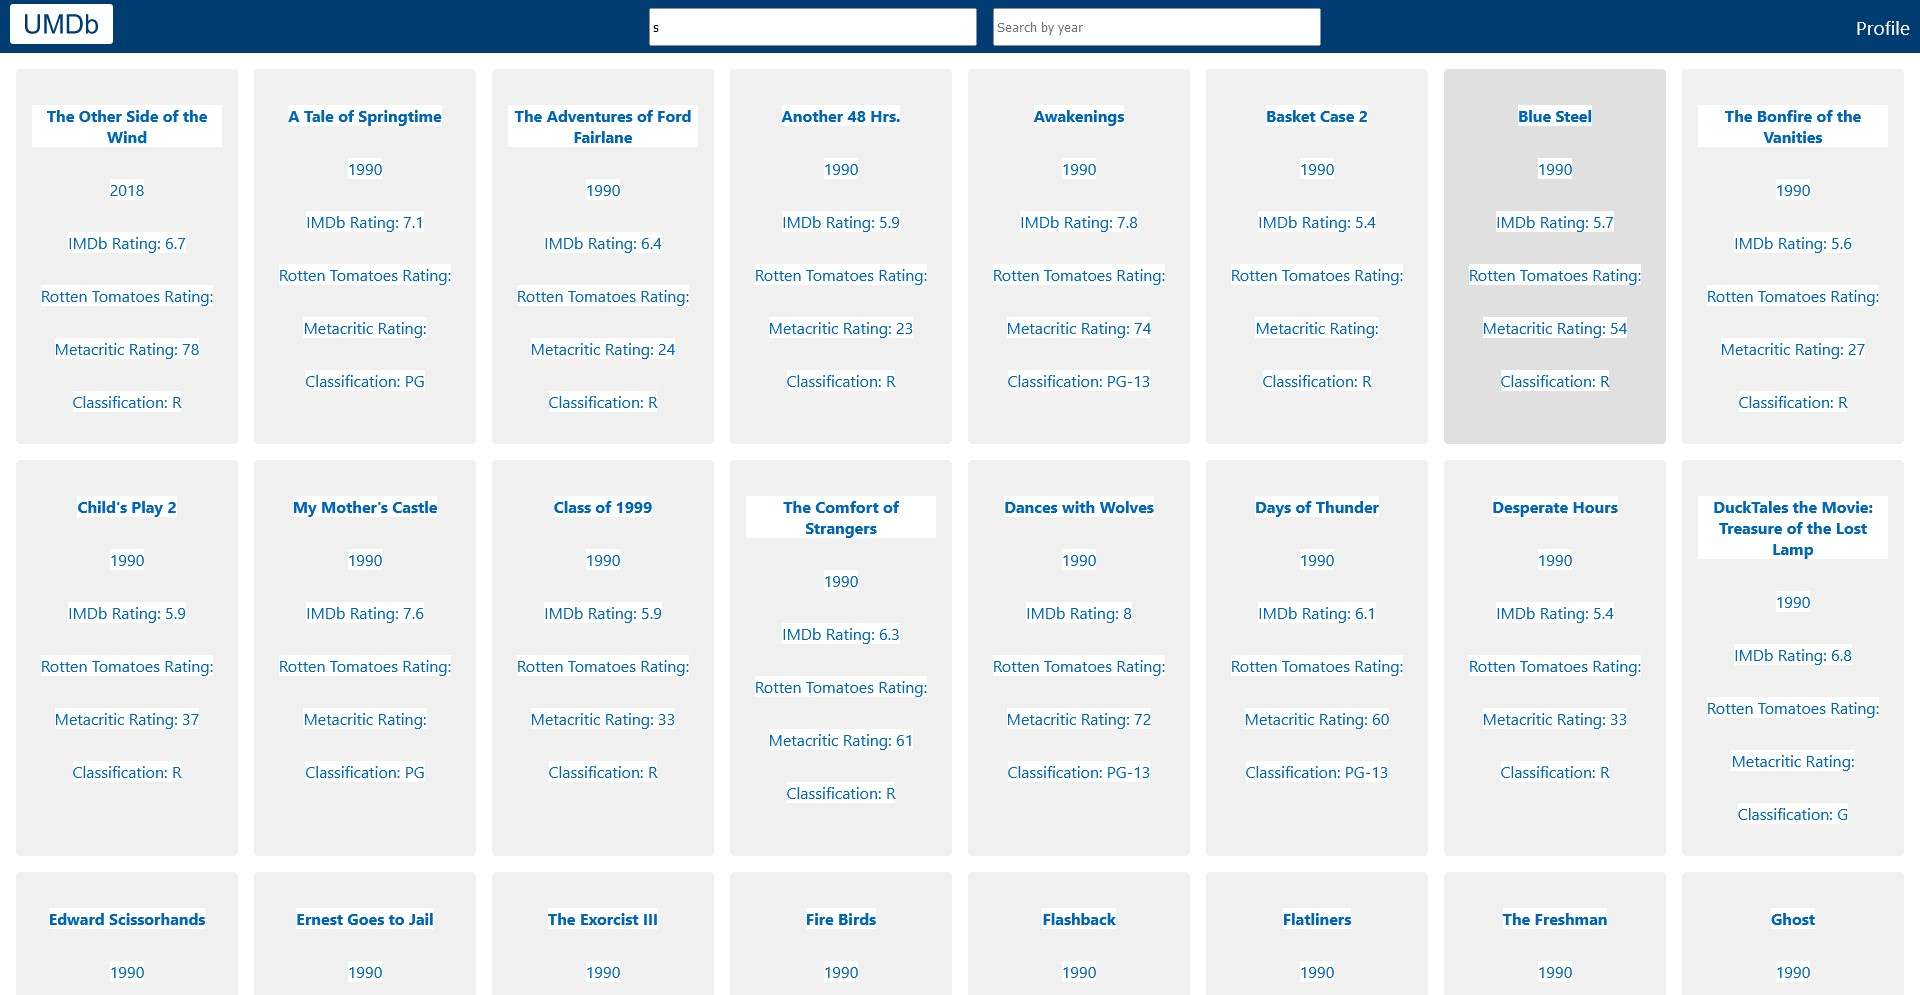
\includegraphics[width=\textwidth]{./figures/Figure12.jpg}}
			  	\captionof{figure}{Another experimental version of the MoviesPage}
			  	\label{fig:figure12}
			\end{center}
		\subsection{Appendix D - Test Plan}
		\label{subsec:appendixD}
			\begin{center}
			  	\fbox{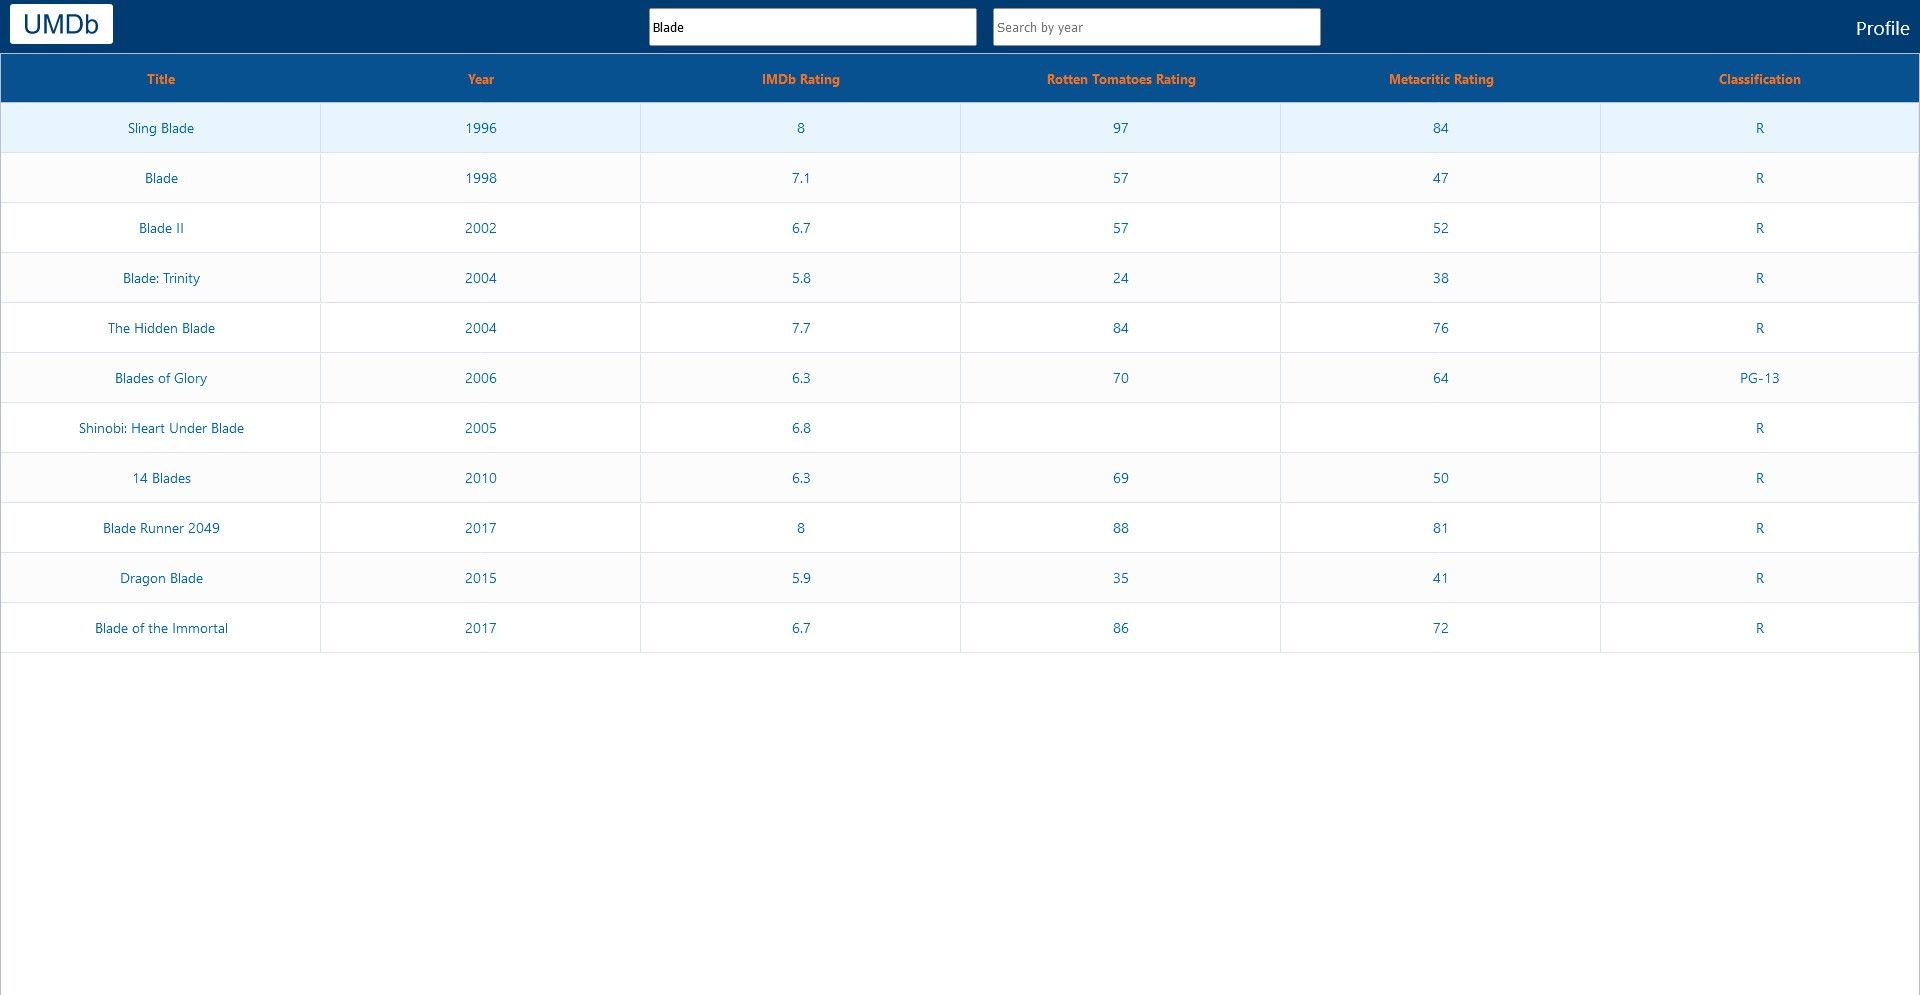
\includegraphics[width=\textwidth]{./figures/Figure13.jpg}}
			  	\captionof{figure}{Test 1 - Search by Title}
			  	\label{fig:figure13}
				\vspace{10pt}
				\fbox{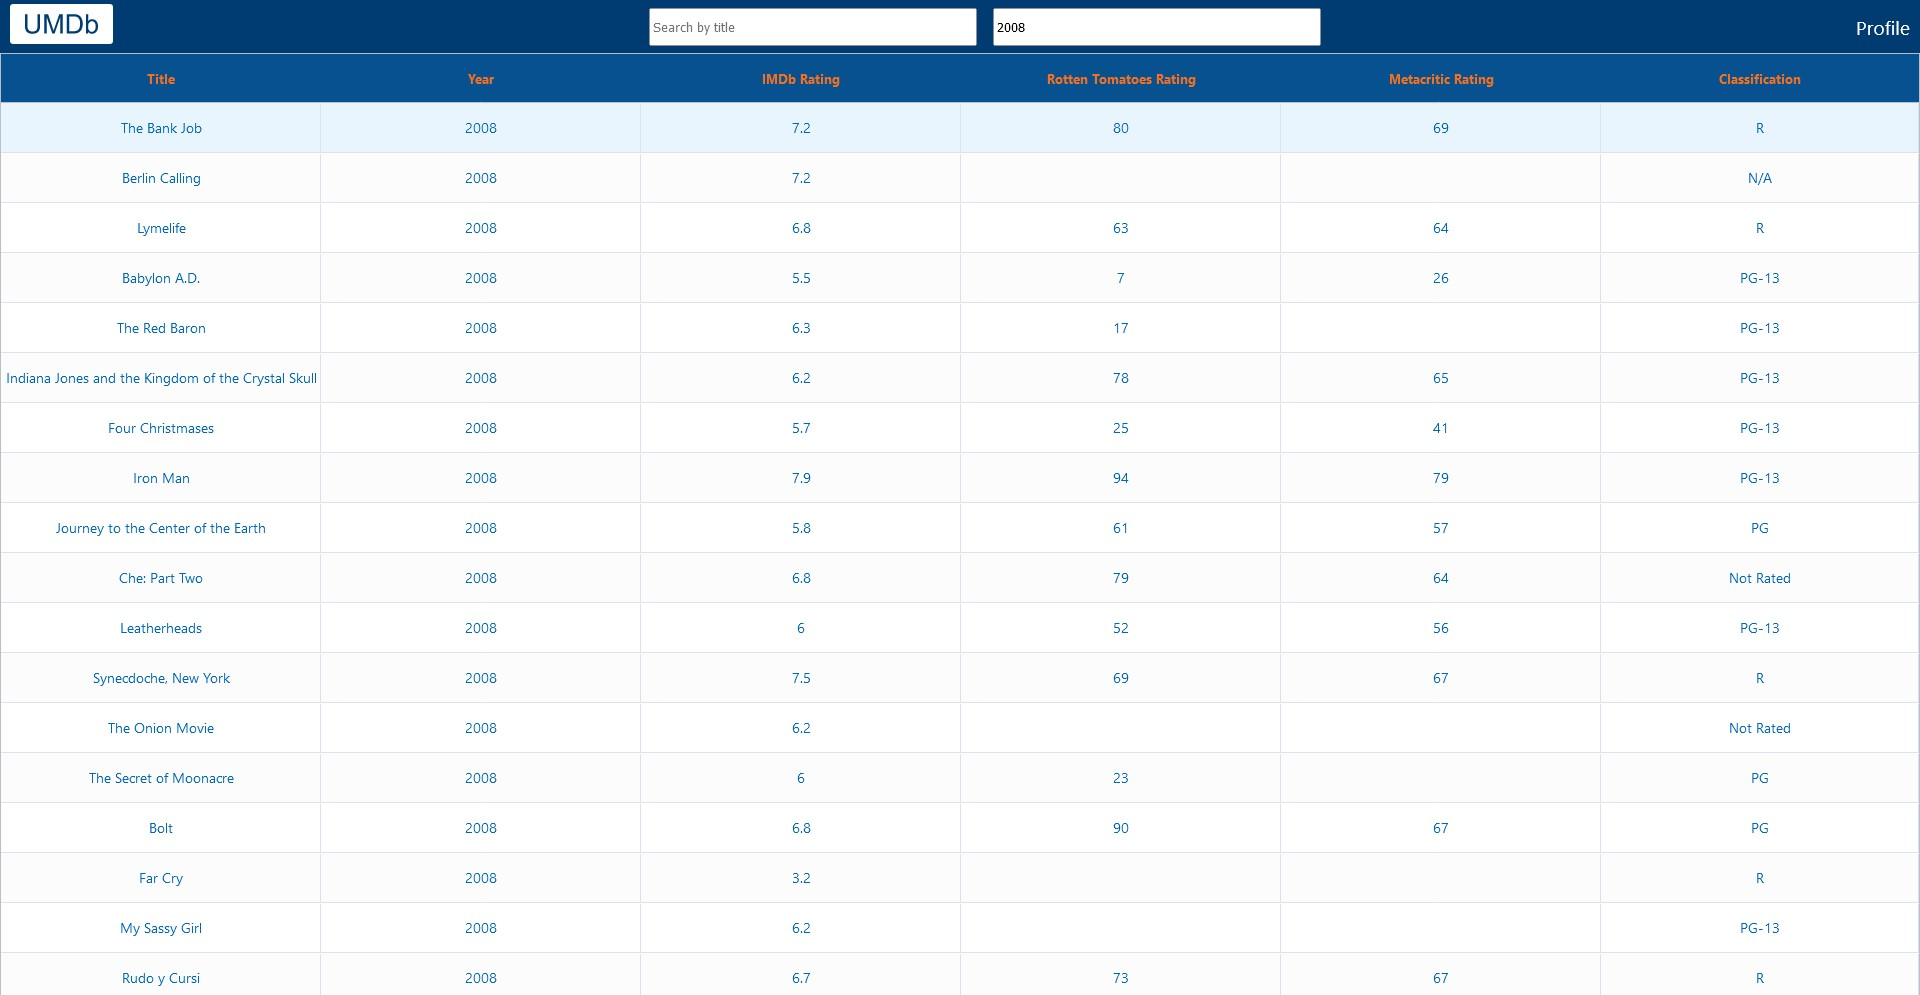
\includegraphics[width=\textwidth]{./figures/Figure14.jpg}}
			  	\captionof{figure}{Test 2 - Search by Year}
			  	\label{fig:figure14}
				\vspace{10pt}
				\fbox{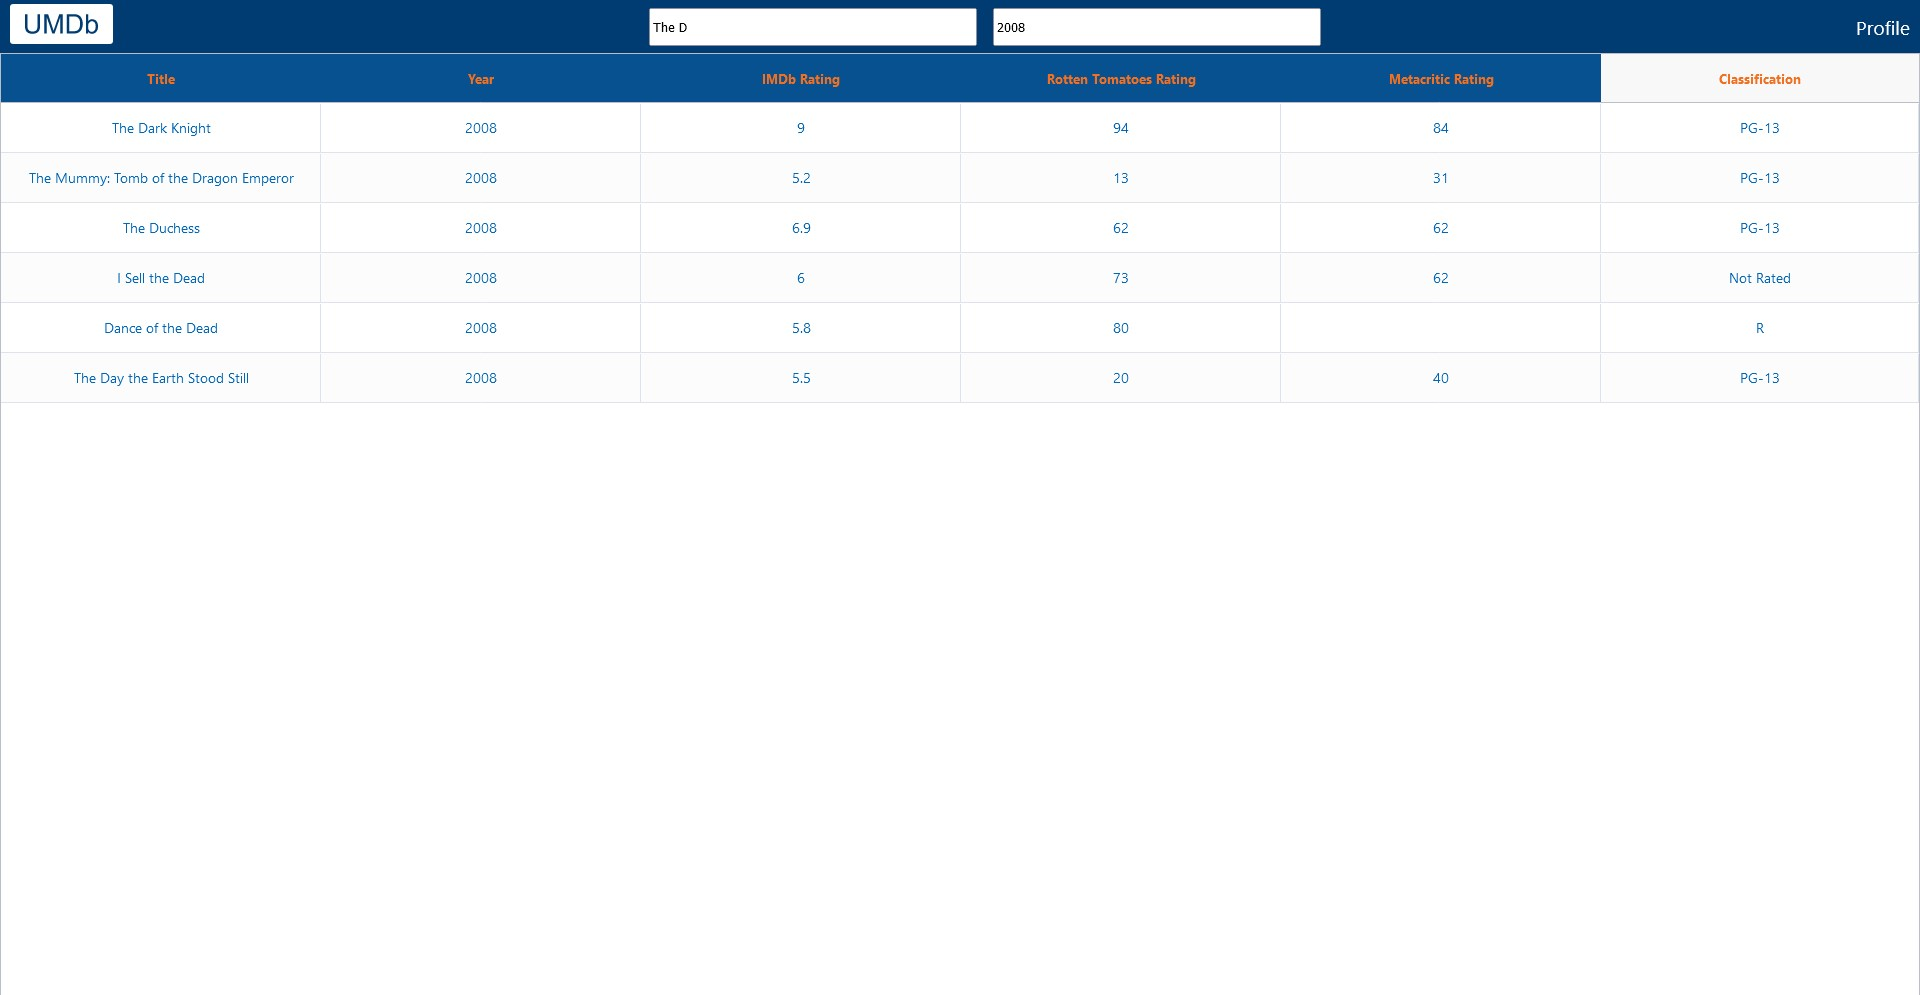
\includegraphics[width=\textwidth]{./figures/Figure15.jpg}}
			  	\captionof{figure}{Test 3 - Search by Title and Year}
			  	\label{fig:figure15}
				\vspace{10pt}
				\fbox{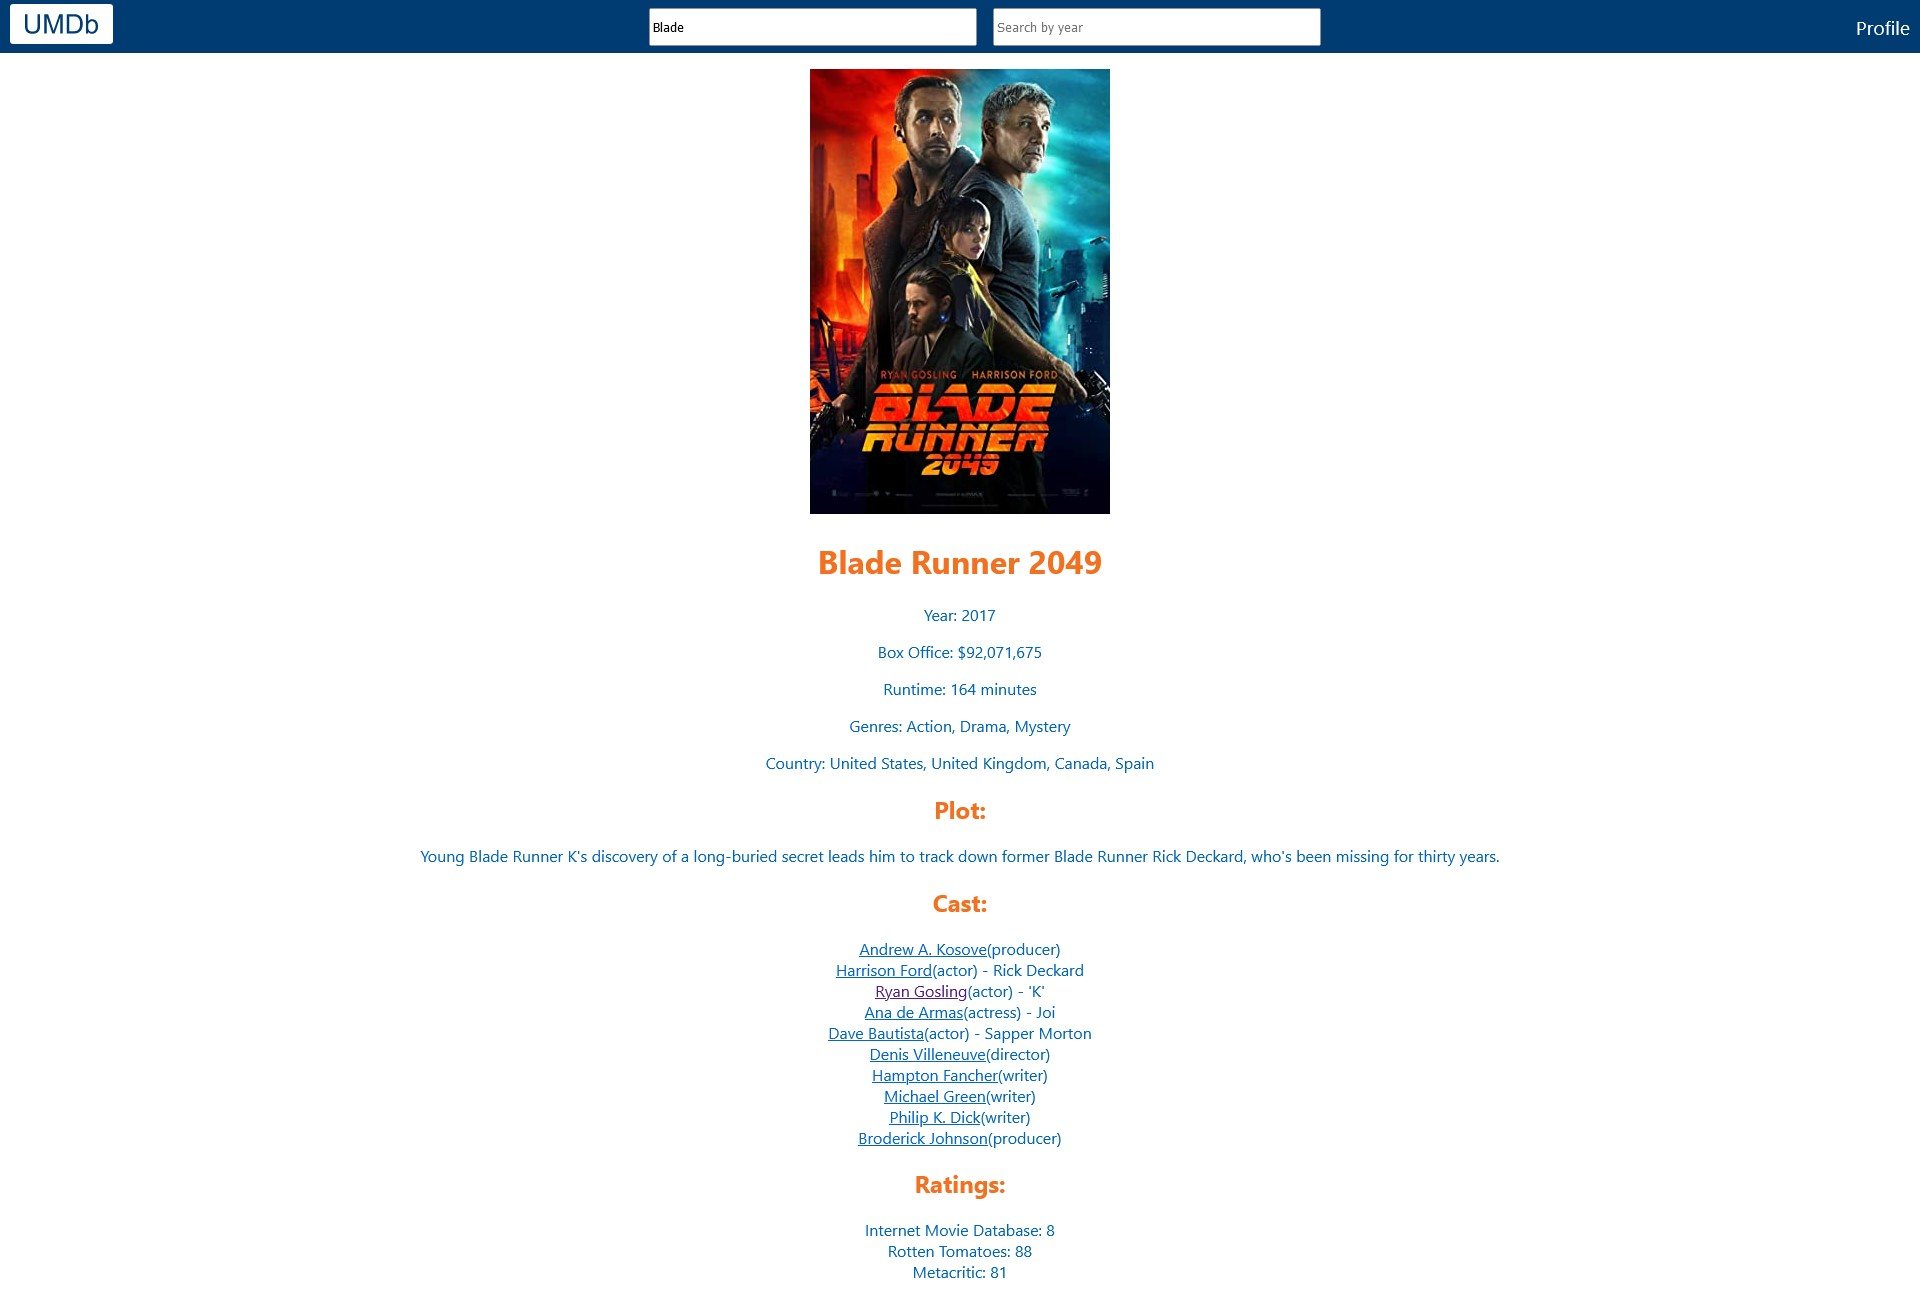
\includegraphics[width=\textwidth]{./figures/Figure16.jpg}}
			  	\captionof{figure}{Test 4 - Click on a Movie}
			  	\label{fig:figure16}
				\vspace{10pt}
				\fbox{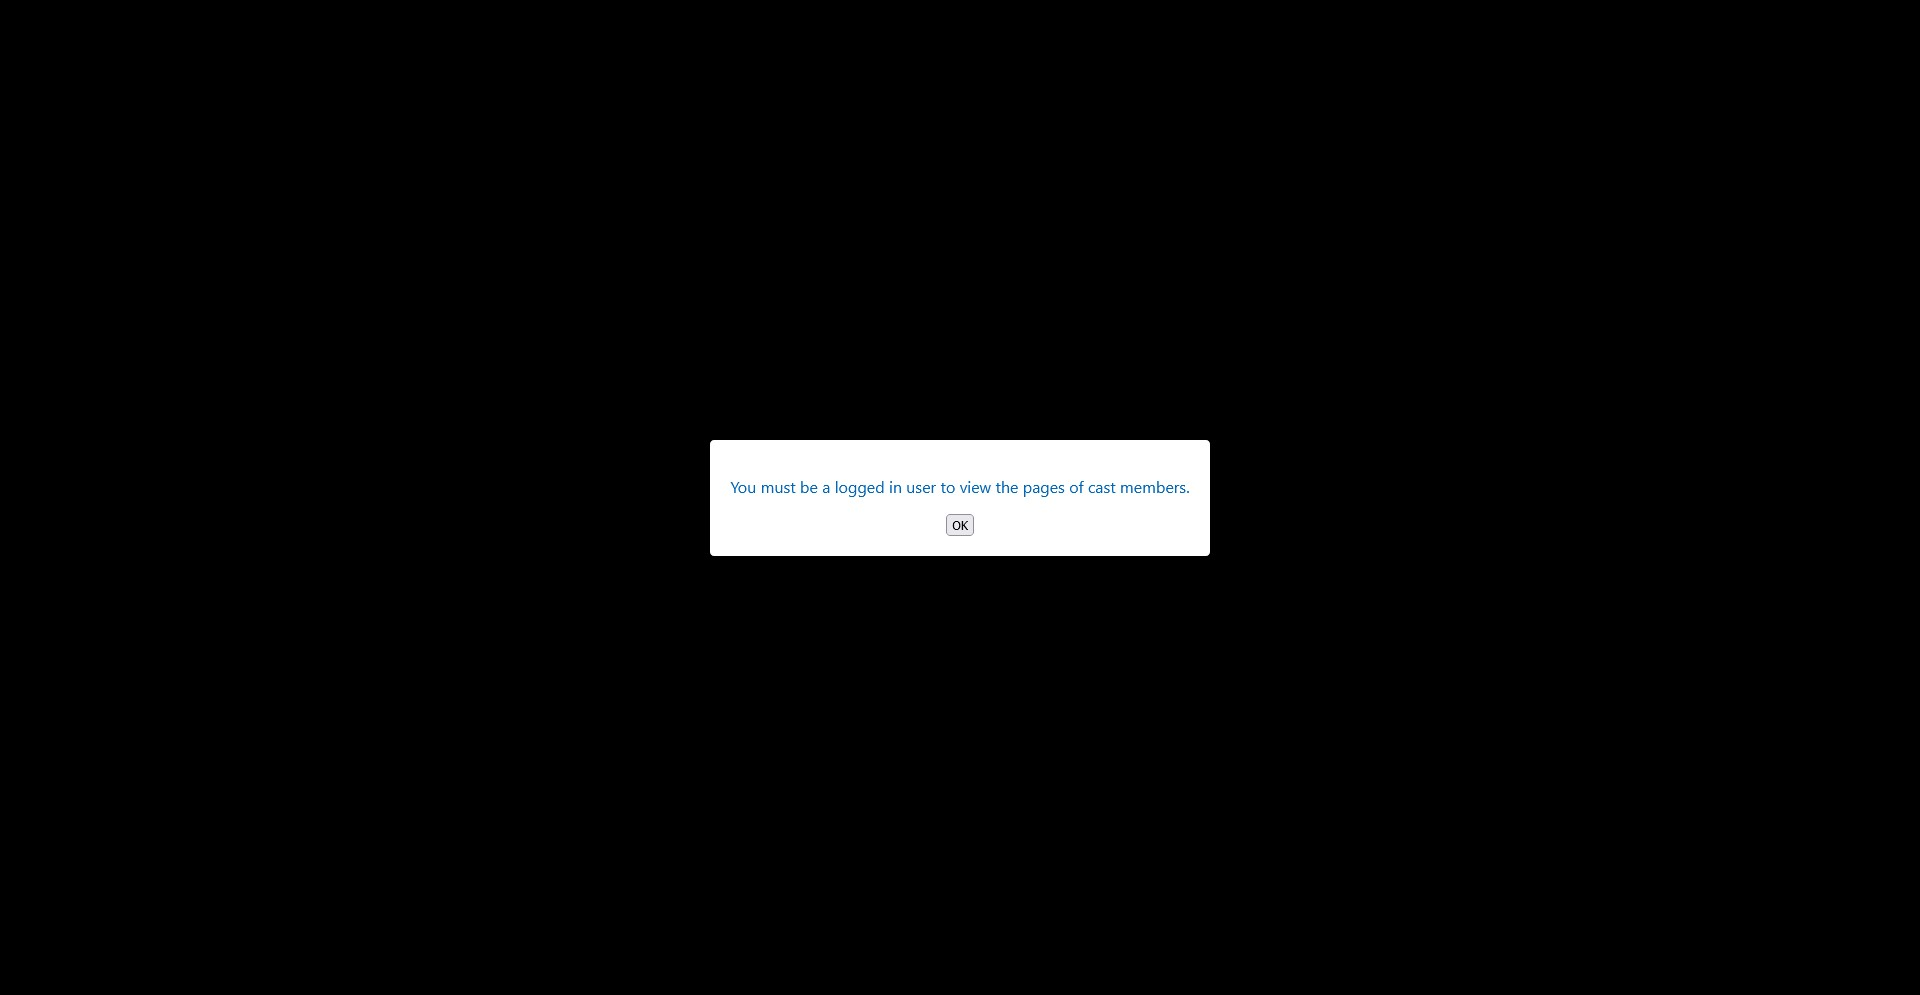
\includegraphics[width=\textwidth]{./figures/Figure17.jpg}}
			  	\captionof{figure}{Test 5 - Click on a Cast Member (Logged Out)}
			  	\label{fig:figure17}
				\vspace{10pt}
				\fbox{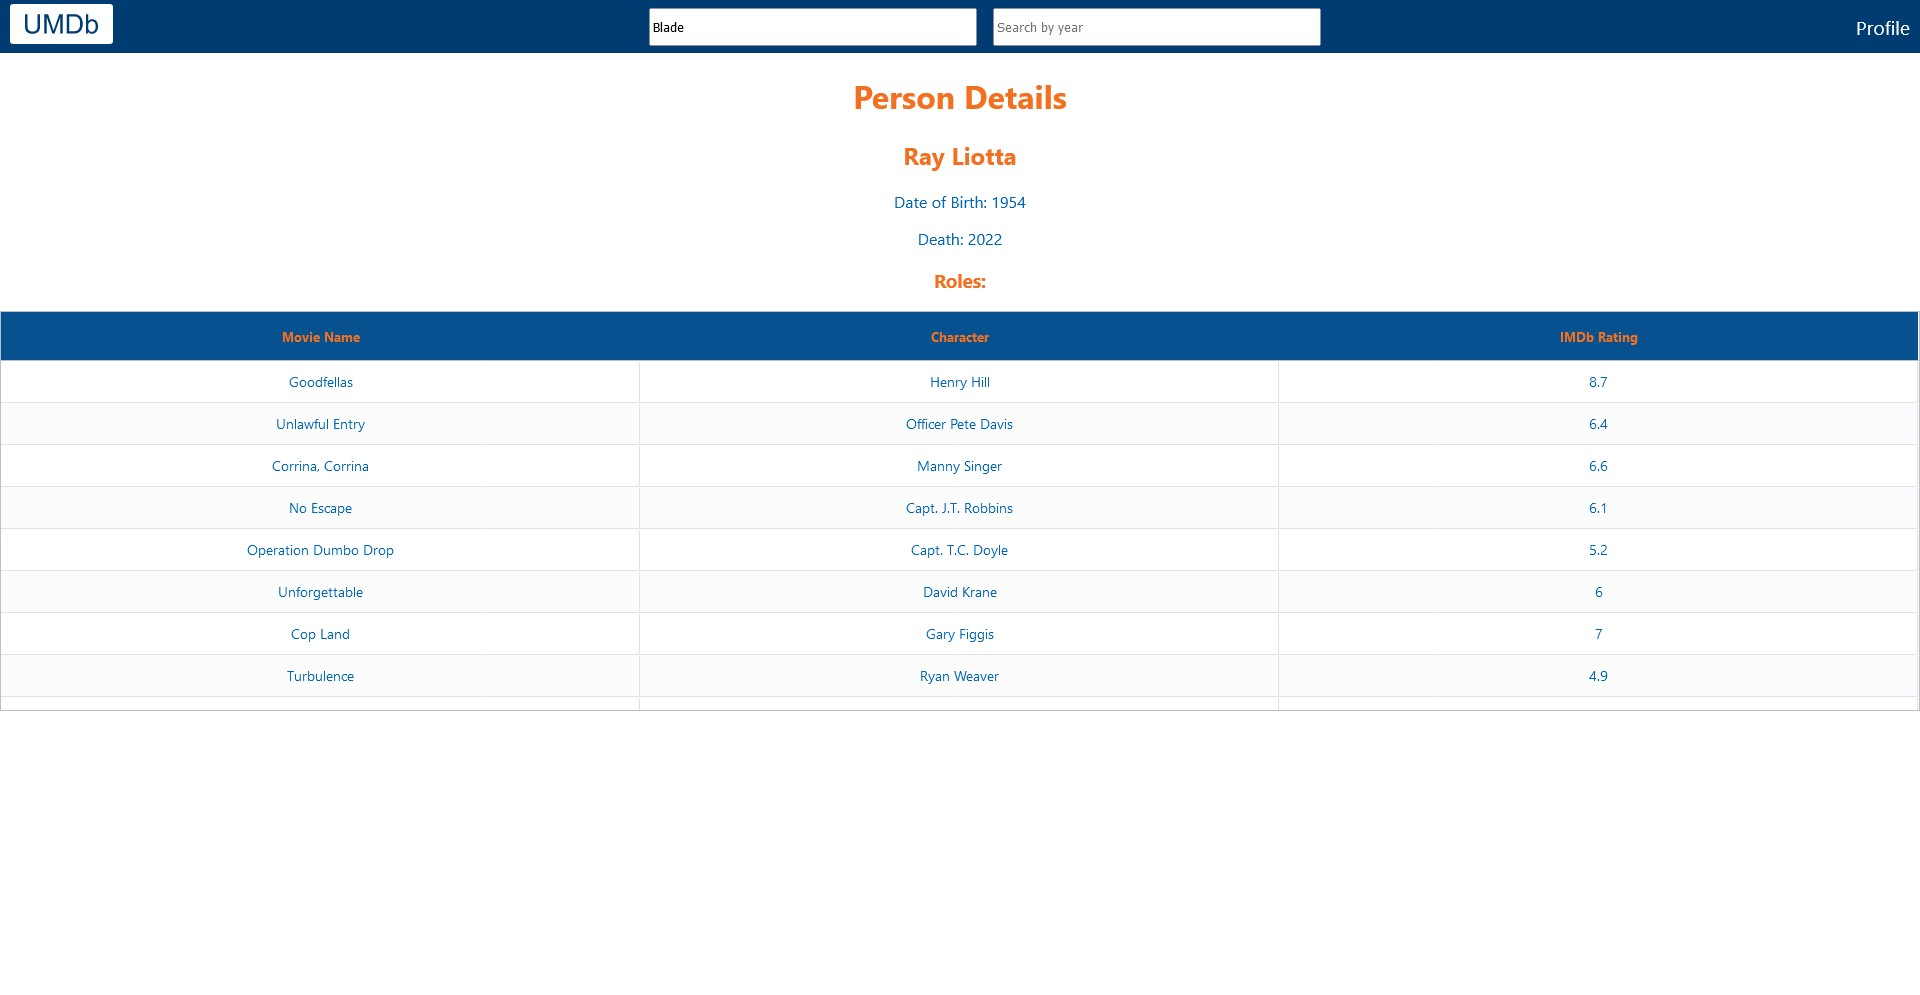
\includegraphics[width=\textwidth]{./figures/Figure18.jpg}}
			  	\captionof{figure}{Test 6 - Click on a Cast Member (Logged In)}
			  	\label{fig:figure18}
				\vspace{10pt}
				\fbox{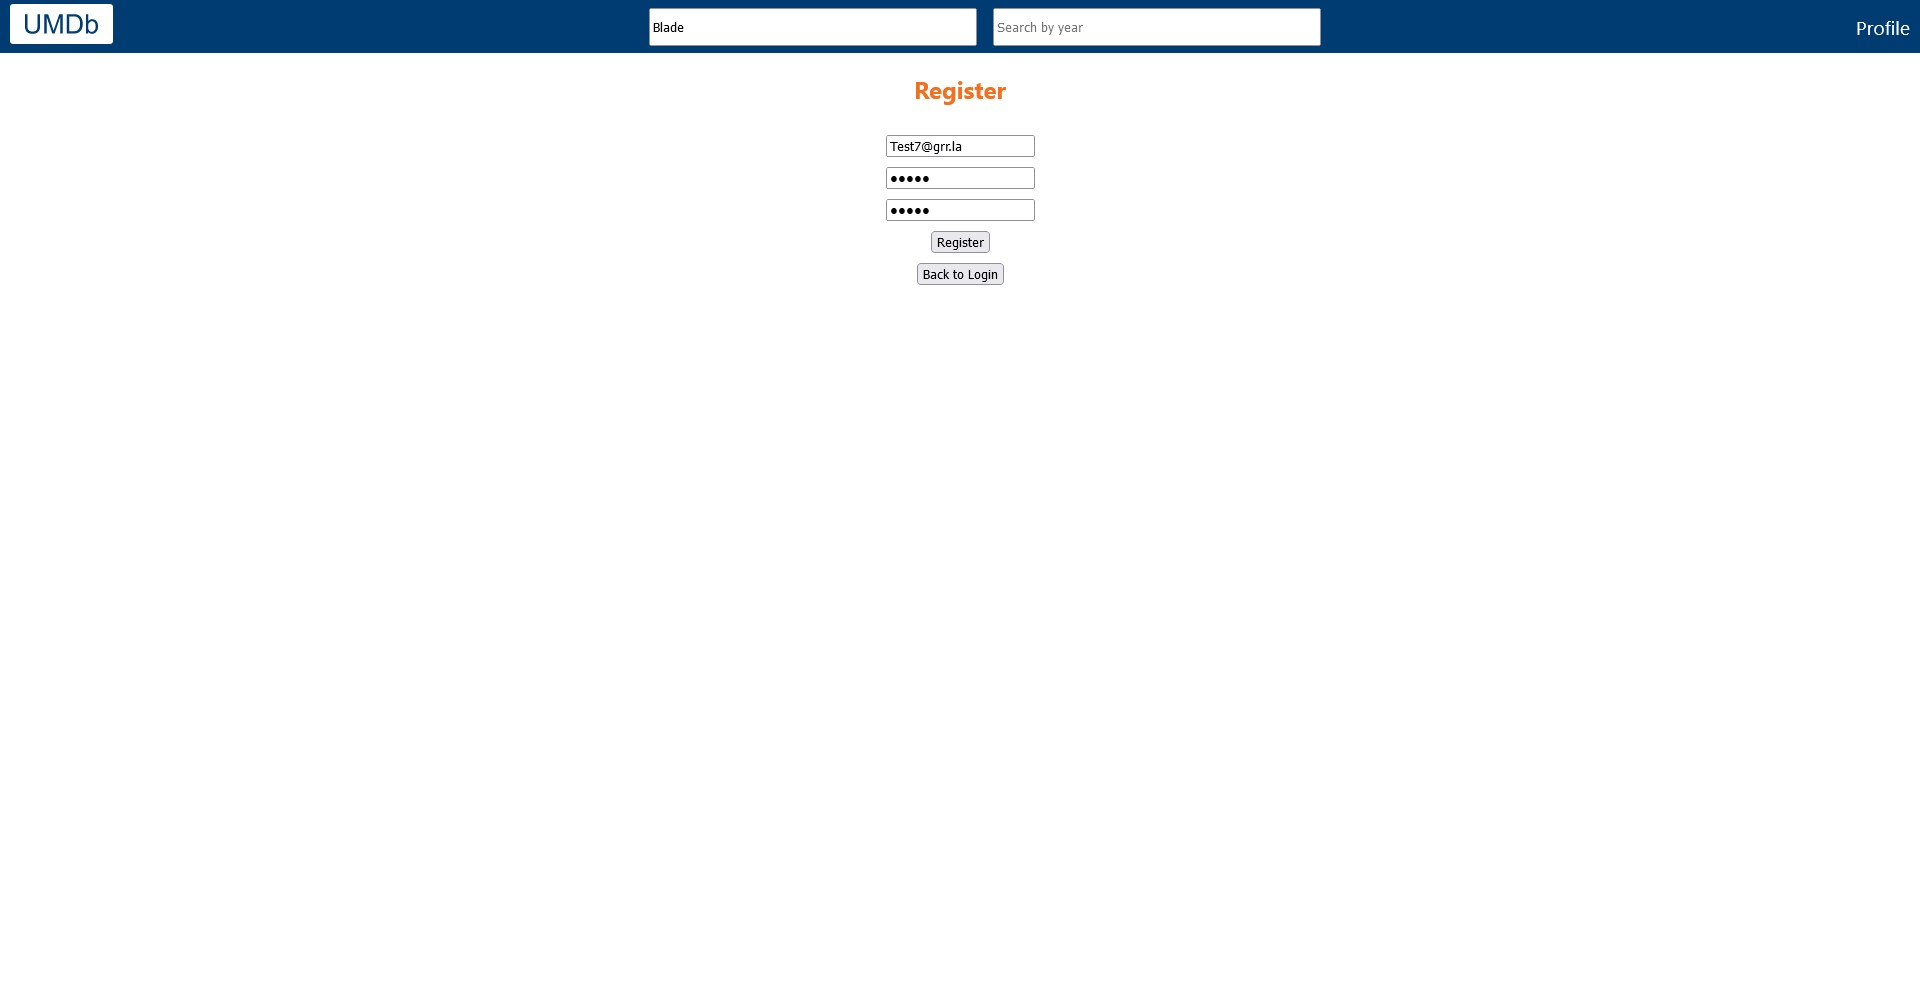
\includegraphics[width=\textwidth]{./figures/Figure19.jpg}}
			  	\captionof{figure}{Test 7 - Register a New User}
			  	\label{fig:figure19}
				\vspace{10pt}
				\fbox{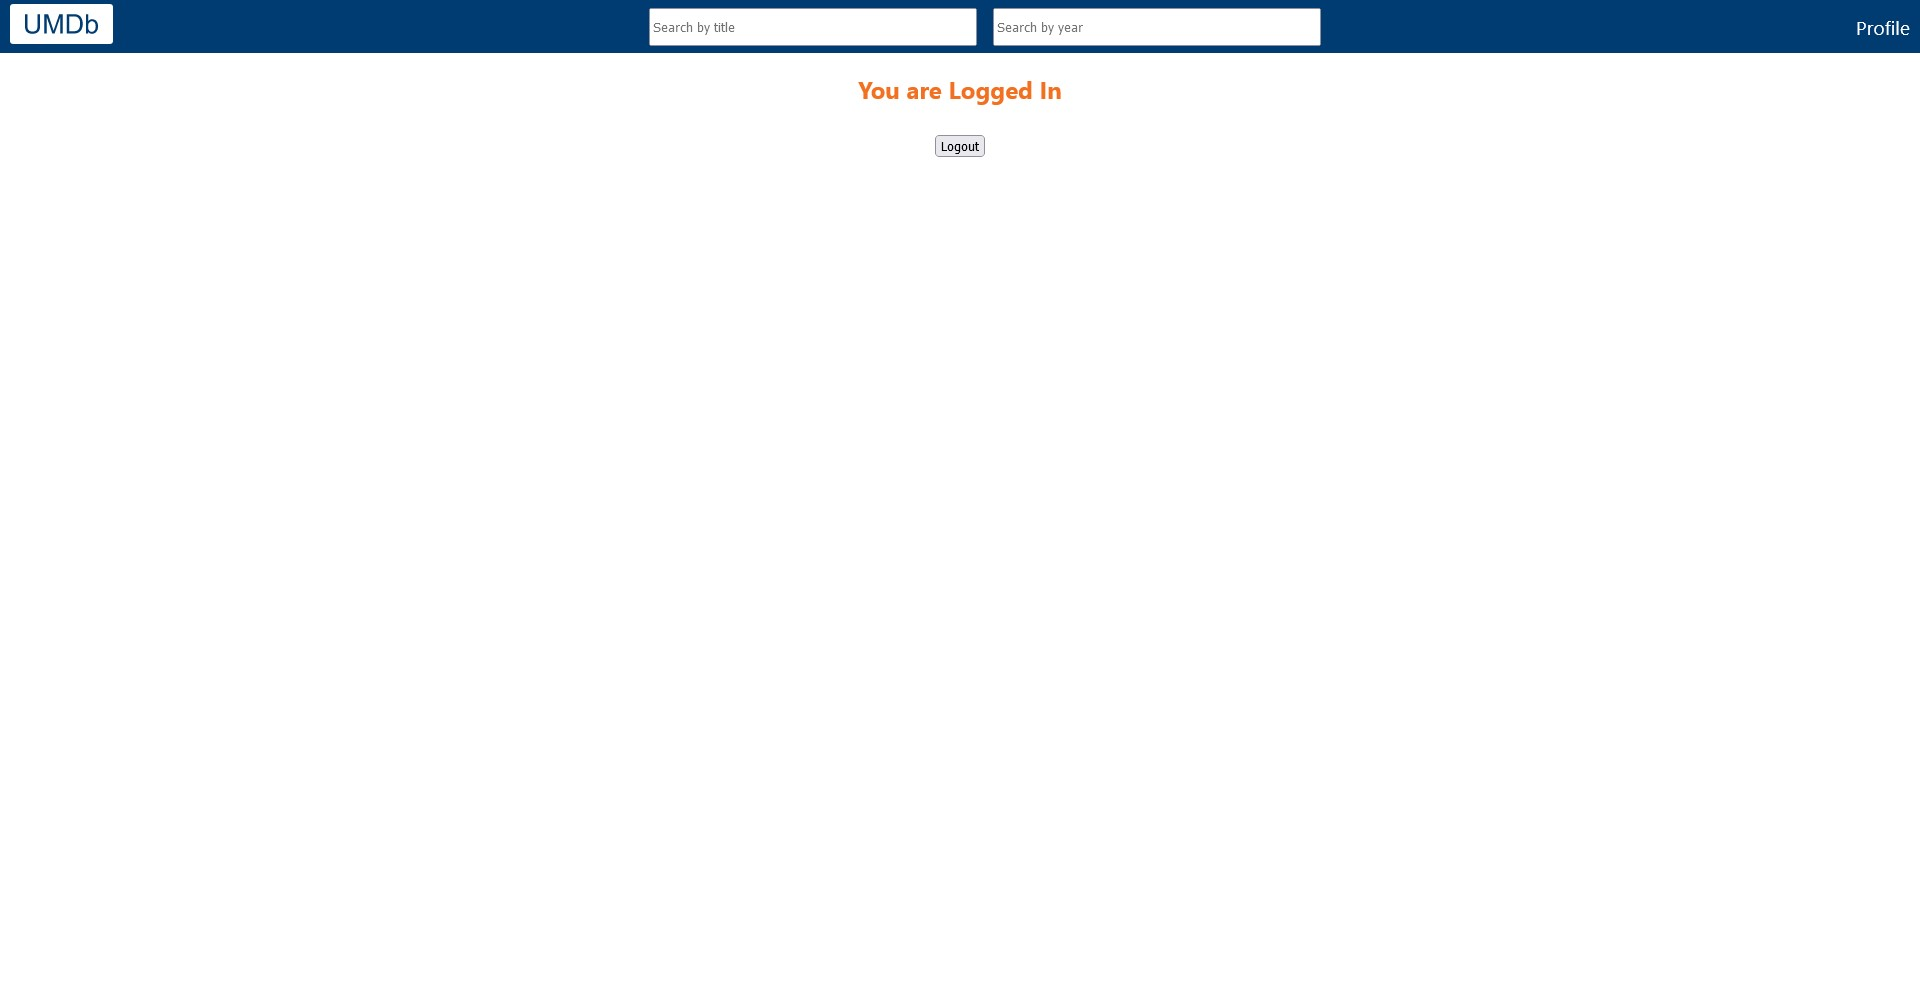
\includegraphics[width=\textwidth]{./figures/Figure20.jpg}}
			  	\captionof{figure}{Test 7 - Logged in as a User}
			  	\label{fig:figure20}
				\vspace{10pt}
				\fbox{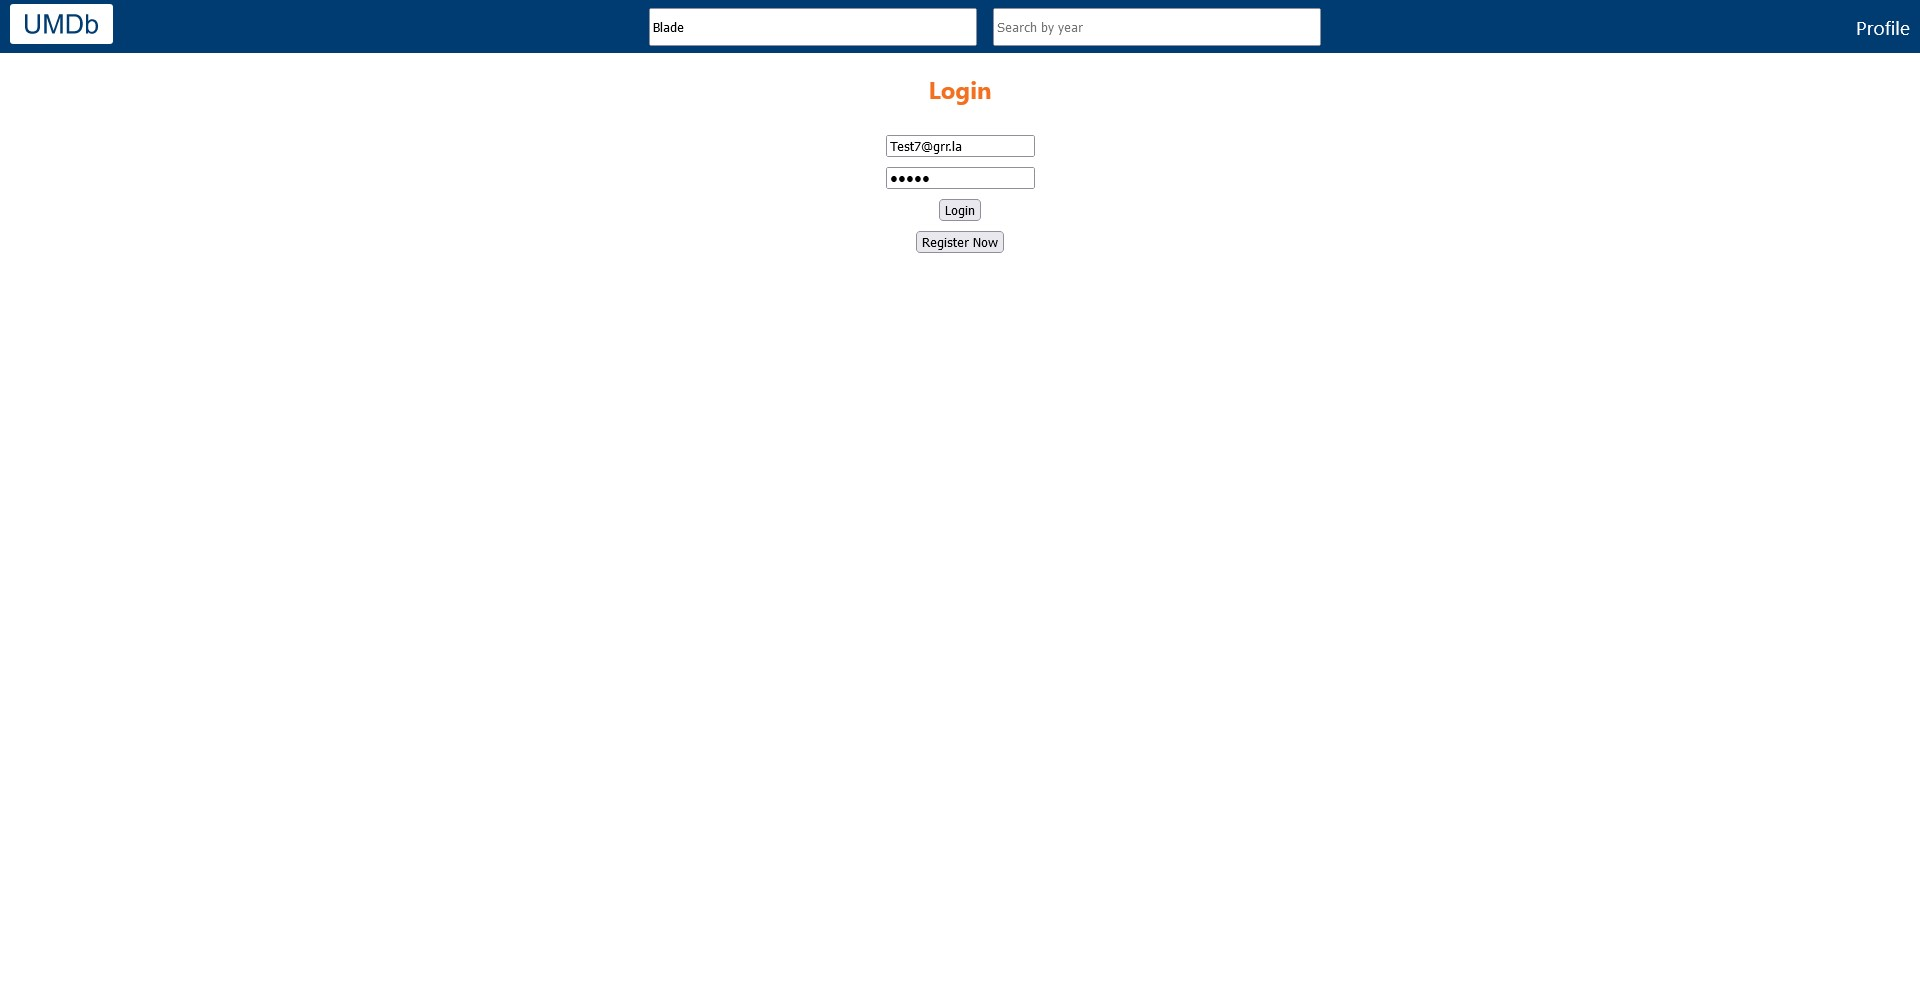
\includegraphics[width=\textwidth]{./figures/Figure21.jpg}}
			  	\captionof{figure}{Test 8 - Login in as User}
			  	\label{fig:figure21}
				\vspace{10pt}
				\fbox{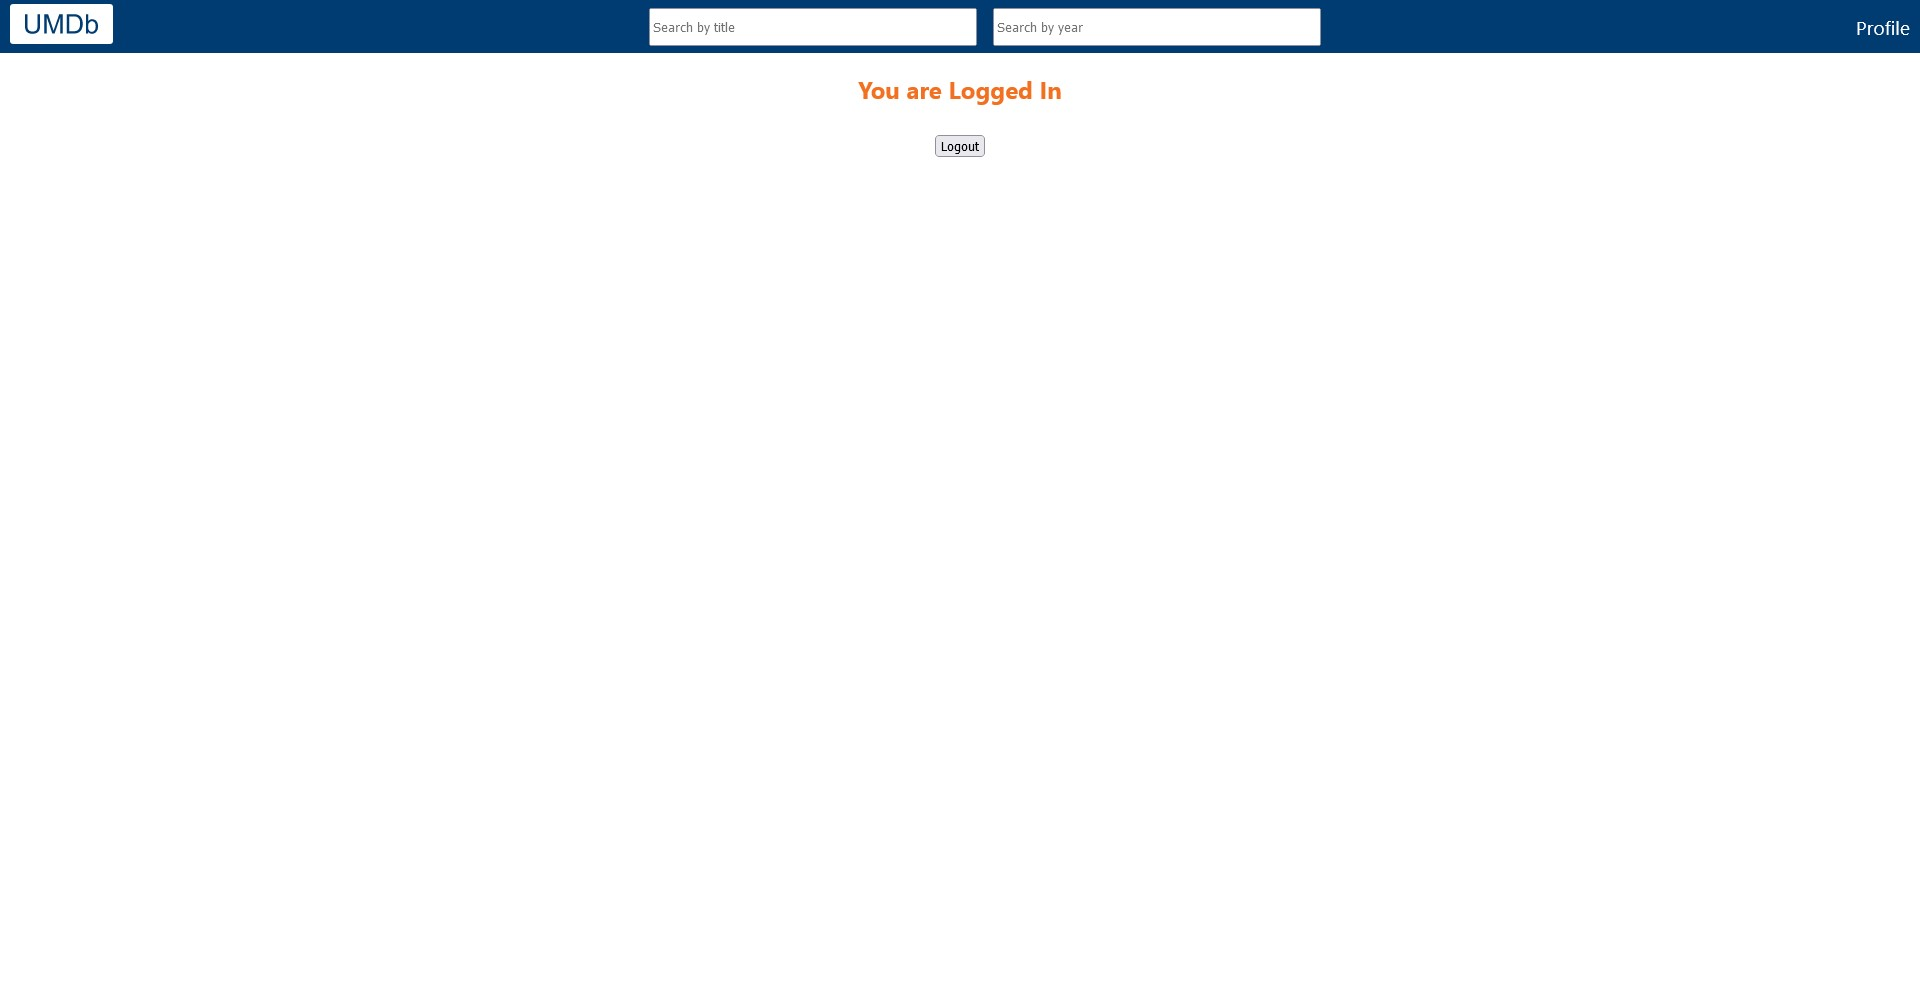
\includegraphics[width=\textwidth]{./figures/Figure22.jpg}}
			  	\captionof{figure}{Test 8 - Logged in as a User}
			  	\label{fig:figure22}
				\vspace{10pt}
				\fbox{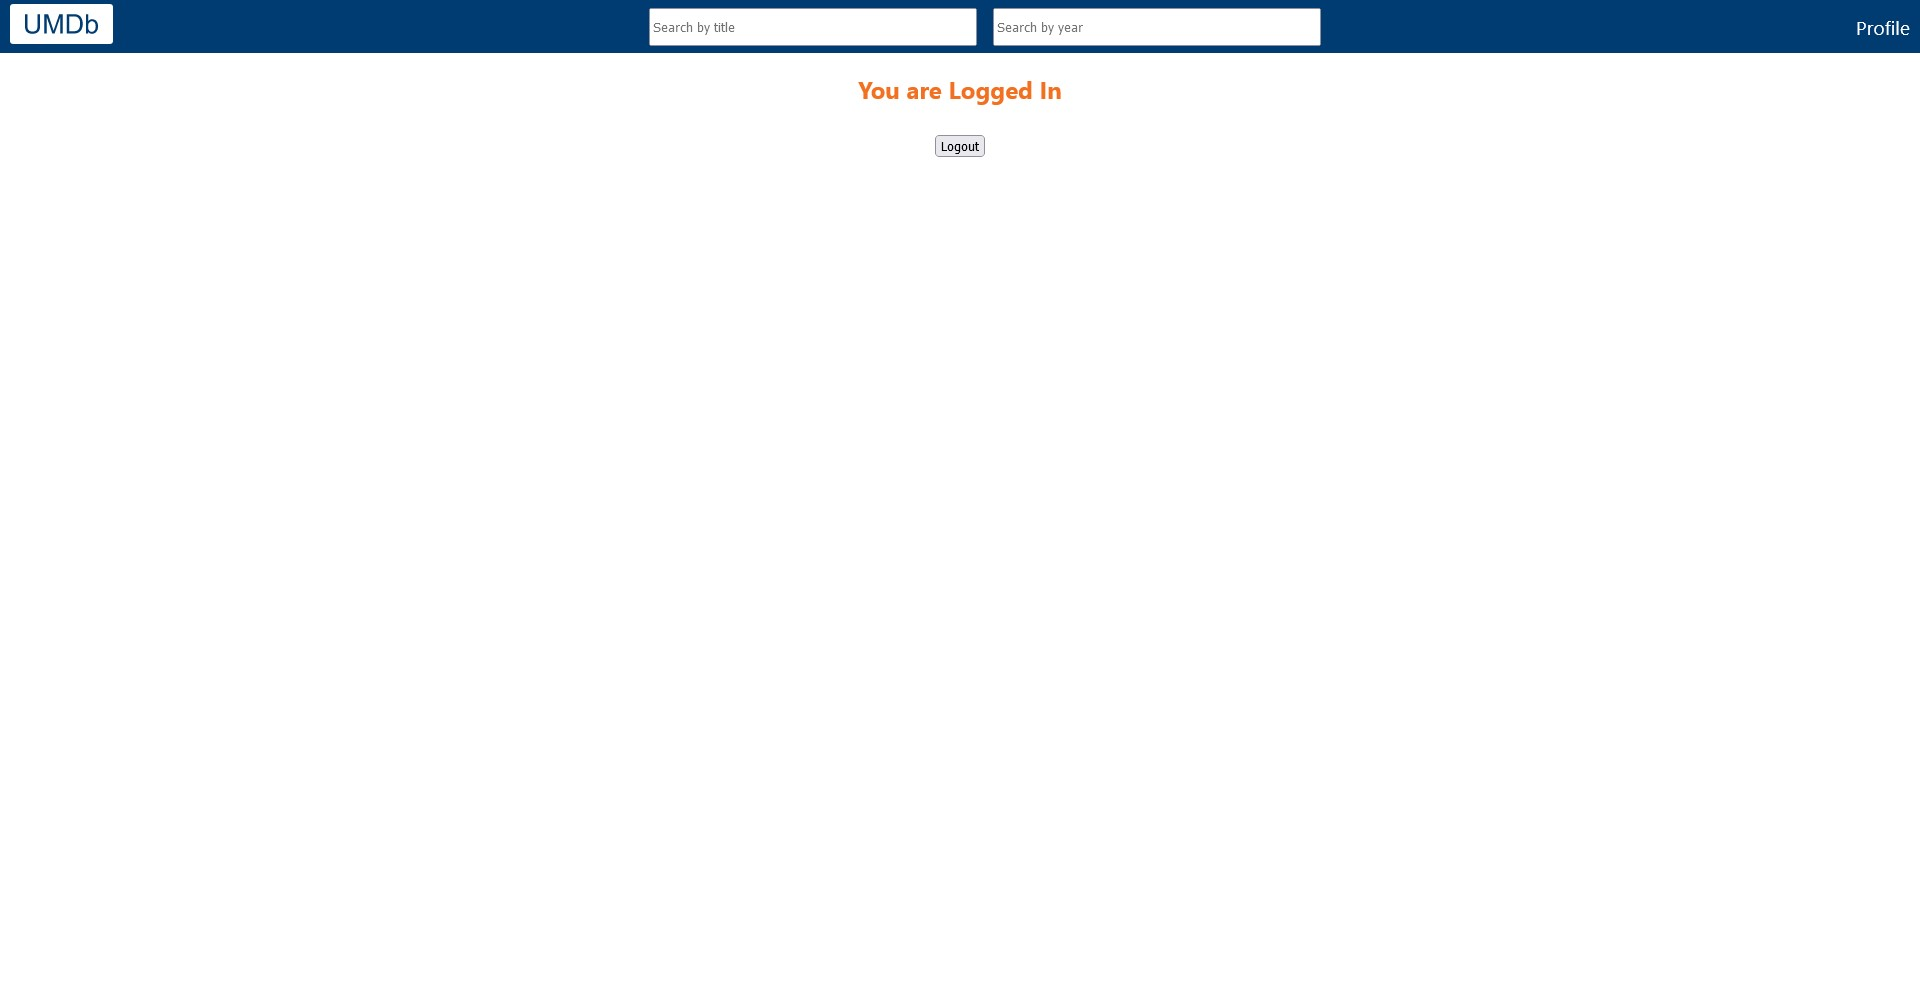
\includegraphics[width=\textwidth]{./figures/Figure23.jpg}}
			  	\captionof{figure}{Test 9 - Ready to Logout}
			  	\label{fig:figure23}
				\vspace{10pt}
				\fbox{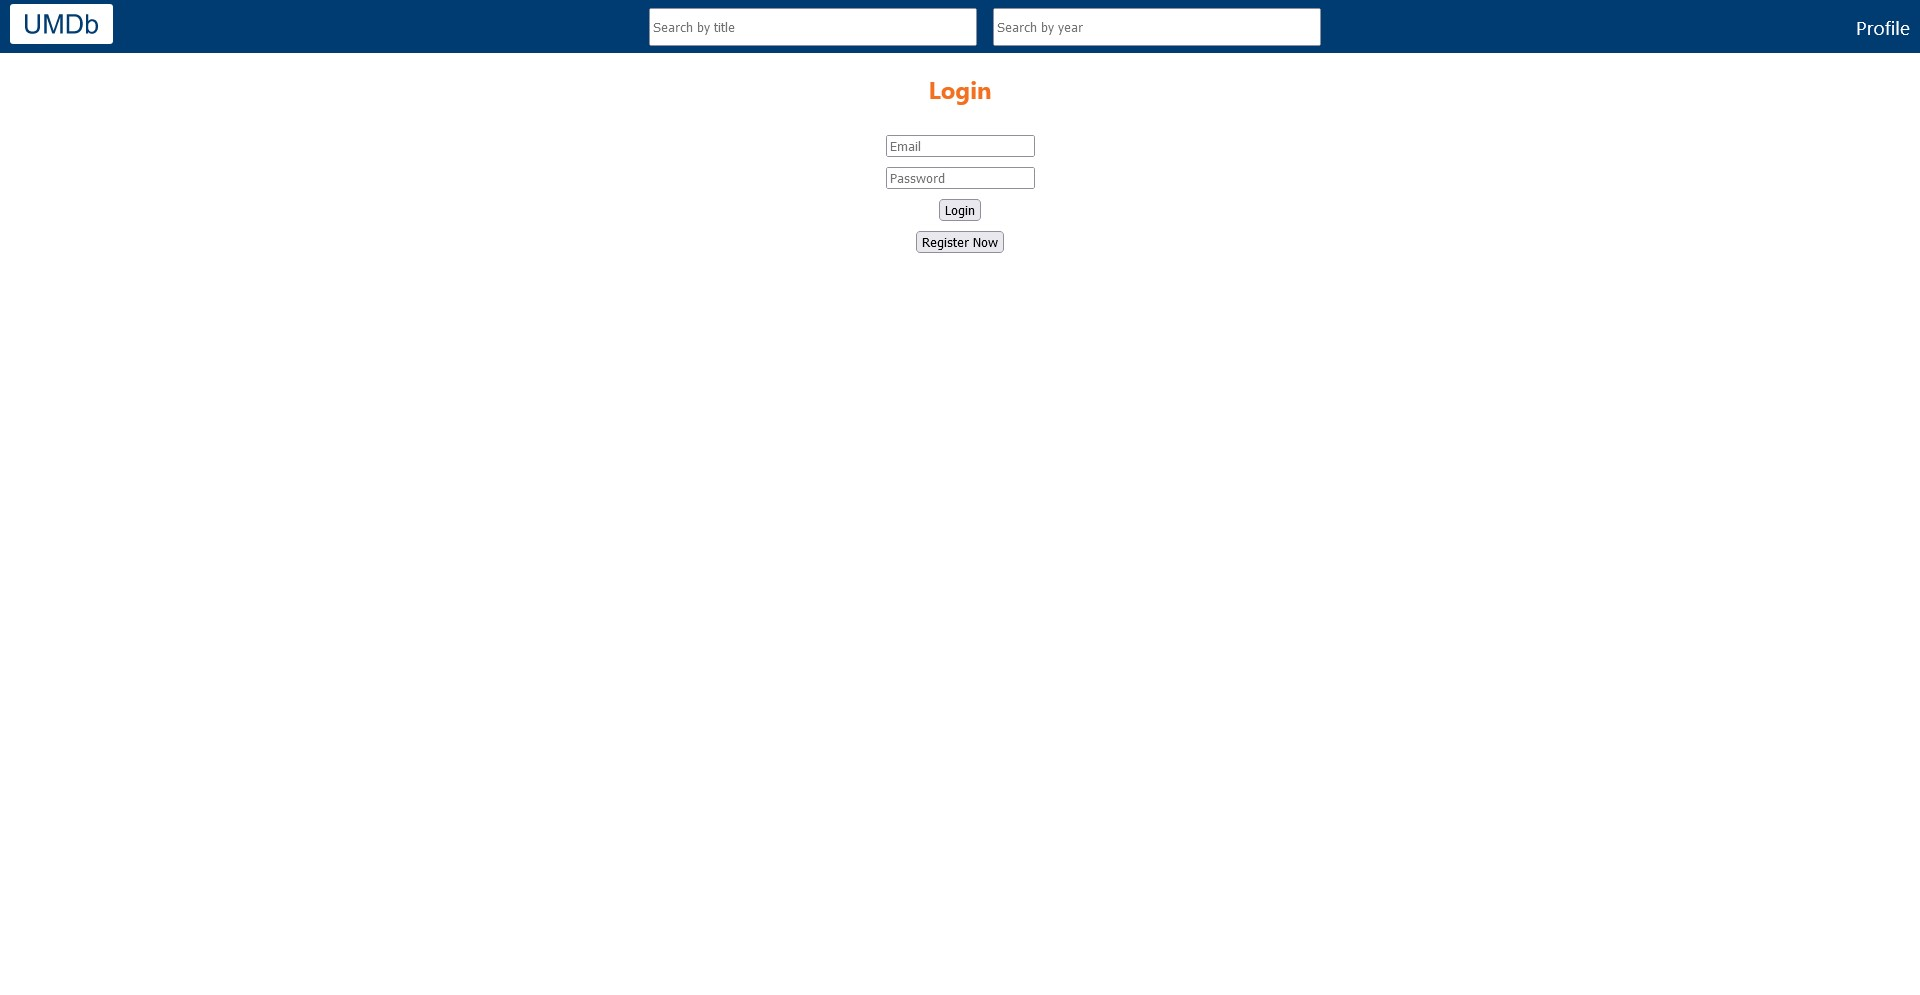
\includegraphics[width=\textwidth]{./figures/Figure24.jpg}}
			  	\captionof{figure}{Test 9 - Logged Out}
			  	\label{fig:figure24}
			\end{center}


\end{document}